\documentclass[11pt,a4paper]{jsarticle}

%%%%%%%%%%%%%%%%%%%%%%%%%
% Packages
%%%%%%%%%%%%%%%%%%%%%%%%%
\usepackage{
	amsmath, % 環境
	amssymb, % 記号
	amsfonts % 特殊文字
}
\usepackage{ascmac}
\usepackage{ulem}
\usepackage{lmodern}
\usepackage{bm}
\usepackage{mathtools, centernot, physics}
\usepackage{enumerate}
% \usepackage{graphicx}
\usepackage[dvipdfmx]{graphicx}
\usepackage{comment} % 複数行をコメントアウトする
\usepackage{url}
\usepackage{array, booktabs, multirow, makecell} % tabular関連
% \usepackage{romannum} % ローマ数字
% \usepackage{xcolor}
\usepackage[dvipdfmx, dvipsnames]{xcolor}
\usepackage{setspace}
\usepackage{float}

%%%%%%%%%%%%%%%%%%%%%%%%%
% Format
%%%%%%%%%%%%%%%%%%%%%%%%%
\setlength{\textwidth}{\fullwidth}
\setlength{\textheight}{40\baselineskip}
\addtolength{\textheight}{\topskip}
\setlength{\voffset}{-0.2in}
\setlength{\topmargin}{0pt}
\setlength{\headheight}{0pt}
\setlength{\headsep}{0pt}

%%%%%%%%%%%%%%%%%%%%%%%%%
% Definitions
%%%%%%%%%%%%%%%%%%%%%%%%%
\newcommand{\alert}[1]{\textbf{\textcolor{red}{#1}}}
\newcommand{\rainn}{\textcolor{blue}{\uline{\ \ \ \ }}}
\newcommand{\sizi}[1]{\textcolor{OliveGreen}{\lbrack #1\rbrack}}

	
\begin{document}


	
\section{目的}
	デジタル画像に対する処理であるフーリエ変換と離散コサイン変換、畳み込みによる低域通過フィルタリングと高域通過フィルタリングを実験により確認し、その処理方法とデジタル画像における周波数特性について理解する。
	
\section{原理}
一般的に、デジタルのフルカラー画像は三次元離散時間信号である。
それは、三つの二次元離散時間信号から成り、それらは赤・緑・青の色成分をそれぞれ表しておりチャンネルと呼ばれる。
その二次元離散時間信号は、縦と横の軸からなり、それぞれの要素は画素と呼ばれ空間的な座標における色成分の大きさを表している。
画素値は、一般的に非符号付き8bit整数で保存されているが、処理する過程では$[0, 1]$の範囲の16bit浮動小数点で扱う場合が多い。
簡単のために、本実験ではフルカラー画像ではなく一チャンネルのみのグレースケール画像について議論する。
以降、全資料においてデジタルのグレースケール画像を単に画像と表記し、また離散時間の表記を省略する。


% 畳み込み
\subsection{畳み込み}
古典的な画像処理手法は、所望の周波数特性を有するフィルタを用いたフィルタリングで実現されている。
フィルタは、二次元信号であり各要素はフィルタ係数を表している。
画像$\mathbf{X}$に対するフィルタ$\mathbf{F}$によるフィルタリングは畳み込み演算$\mathbf{X}\ast\mathbf{F}$で実現され、以下の式で定義されている。
%%%%%%%%%%%%%%%%%%
\begin{equation}
	y_{ij} = \sum^{k_i}_{m=-k_i}\sum^{k_j}_{n=-k_j}
	x_{(i+m)(j+n)}\times f_{-m\ -n}
	\label{eq:Conv}
\end{equation}
%%%%%%%%%%%%%%%%%%
ここで、$y_{ij}$と$x_{ij}$、$f_{ij}$は出力画像$\mathbf{Y}$と$\mathbf{X}$、$\mathbf{F}$の$(i,j)$要素を表し、$2k_i+1$と$2k_j+1$は$\mathbf{F}$の縦横方向の長さをそれぞれ表している。
つまり$\mathbf{F}$は、簡単のために縦横奇数の長さを持つと仮定しており、中心座標を$(0,0)$として中心から上下左右にそれぞれ$k_i$と$k_j$の要素数を持つことを表している。


% DFTと周波数特性について
\subsection{周波数解析}\label{sec:Fourier}
離散時間信号の周波数解析には離散フーリエ変換（DFT: Discrete Fourier transform）を用いるのが一般的である。
長さ$N$を持つ一次元信号$\bm{x}$のDFTは以下の式で定義されている。
%%%%%%%%%%%%%%%%%%
\begin{equation}
	X(\omega)=\sum^{N-1}_{n=0}x_n\exp
	\left(-j\omega n\right)
	\label{eq:DFT}
\end{equation}
%%%%%%%%%%%%%%%%%%
ここで、$x_n$は$\bm{x}$の$n$番目要素を表し、$\omega=2\pi k/N$である。
定義より、$X(\omega)$は$2\pi$の周期関数となり、$\bm{x}$の要素が実数値である場合、その周波数振幅特性$|X(\omega)|$と位相特性$\angle X(\omega)$は偶関数と奇関数になる。
よって、$|X(\omega)|$は$[0, \pi]$の範囲を確認すれば良い。

二次元信号である画像$\mathbf{X}$の周波数解析には二次元DFTを用いる。
二次元DFTは、式(\ref{eq:DFT})をそのまま二次元に拡張した以下の式で定義されている。
%%%%%%%%%%%%%%%%%%
\begin{equation}
	X(\omega_i, \omega_j)=
	\sum^{M-1}_{m=0}\sum^{N-1}_{n=0}x_{mn}
	\exp\left\{-\left(j\omega_i m+j\omega_j n\right)\right\}
	\label{eq:2DDFT}
\end{equation}
%%%%%%%%%%%%%%%%%%
ここで、各変数は式(\ref{eq:Conv})と(\ref{eq:DFT})と同様に定義されている。
$|X(\omega_i, \omega_j)|$は、$|X(\omega)|$と同様に$2\pi$の周期関数であり原点対称性を持つが、四象限対称ではないので、各変数の$[-\pi, \pi]$の範囲を確認する必要がある。


% アップ・ダウンサンプリングと周波数振幅特性
\subsection{アップサンプリングとダウンサンプリングと周波数振幅特性}
\label{sec:UpDonwsampling}
長さ$N$を持つ一次元信号$\bm{x}$に対して、各要素間に$0$を挿入して信号長を大きくする処理をアップサンプリングと呼び、等間隔に要素を間引いて信号長を小さくする処理をダウンサンプリングと呼ぶ。
$\bm{x}$を倍率$\gamma$でアップサンプリングした結果を$\bm{y}$とすると以下の式で定義されている。
%%%%%%%%%%%%%%%%%%
\begin{equation}
	y_n=\left\{
	\begin{array}{ll}
		x_{m}&\rm{if}\quad \bmod(n, \gamma) =0\\
		0&otherwise
	\end{array}
	\right.
\end{equation}
%%%%%%%%%%%%%%%%%%
ここで、$\gamma$は一般的に$1$より大きい整数であり、$m={\rm div}(n, \gamma)$、$n=0,1,\cdots,\gamma N$、${\rm div}$と$\bmod$は第一引数を第二引数で割ったときの商と余りを計算する関数をそれぞれ表している。
この場合、$\bm{y}$の信号長は$\gamma N$となる。
また、$\bm{x}$を倍率$\gamma$でダウンサンプリングした結果を$\bm{z}$とすると、$\bm{z}$の信号長は$N/\gamma$となり以下の式で定義されている。
%%%%%%%%%%%%%%%%%%
\begin{equation}
	z_n=x_{n\times\gamma}
\end{equation}
%%%%%%%%%%%%%%%%%%

アップサンプリングとダウンサンプリング後の信号$\bm{y}$と$\bm{z}$をDFTするとそれぞれ$X(\gamma\omega)$と$X(\omega/\gamma)$となる。
アップサンプリングの場合は、$Y(1)$の周波数特性が$X(\gamma)$と等価となるので、元の信号の周波数特性$X(\omega)$が周波数軸上において倍率$\gamma$で縮められた周波数特性に変換されたとみなせる。
一方ダウンサンプリングの場合は、周波数軸上において倍率$\gamma$で引き延ばされたとみなせる。
つまり、時間軸上で引き延ばされる処理は周波数軸上で縮められており、逆もまた同様である。
また、\ref{sec:Fourier}項で示したことと同様に、二次元信号の場合は、縦横それぞれの軸に対して上記処理が可能であり、周波数解析もそれらの軸に沿って収縮と拡張がされる。


% DCTについて
\subsection{離散コサイン変換}\label{sec:DCT}
離散コサイン変換（DCT: Discrete cosine transform）は、DFTの一種であり、実数値での高速処理が実現できるため、画像符号化方式のJPEG等で広く用いられている。
\ref{sec:Fourier}で示したとおり、周波数解析にはDFTを用いるが複素数値の処理となるため、計算量が多く時間がかかるのが欠点である。
DCTは、対象となる信号を対称に拡張しそれにDFTを適用して、対称性を考慮して展開すると虚部が打ち消し合うことから実数値演算として導出される。
DCTは、拡張の仕方により離散サイン変換も含めて四タイプが存在しているが、広く用いられているのはタイプ$2$のものである。
タイプ$2$のDCTの変換行列$\mathbf{D}$は以下の式で定義されている。
%%%%%%%%%%%%%%%%%%
\begin{equation}
	d_{ij}=\sqrt{\frac{2}{M}}\ 
	c_ic_j\cos\left(
	\frac{i(j+1/2)\pi}{M}
	\right)
	\label{eq:DCT}
\end{equation}
%%%%%%%%%%%%%%%%%%
ここで、$d_{ij}$は$\mathbf{D}$の$(i,j)$要素（$i,j=0,1,\cdots,M-1$）を表し、$M$は$\mathbf{D}$のサイズ、$c_k$は係数をそれぞれ表している。
$c_k$は、$\mathbf{D}$が正規直交行列となるために、以下のように定義されている。
%%%%%%%%%%%%%%%%%%
\begin{equation*}
	c_k=\left\{
	\begin{array}{ll}
		1/\sqrt{2}&\mathrm{if}\quad k=0\\
		1&otherwise
	\end{array}
	\right.
\end{equation*}
%%%%%%%%%%%%%%%%%%
よって、${\mathbf D}^{T}\mathbf{D}=\mathbf{I}$である。
ここで、上付きの$T$は転置を表し、$\mathbf{I}$は単位行列をそれぞれ表している。
サンプル数$M$の一次元信号$\bm{x}$をDCTするには、$\bm{y}=\mathbf{D}\bm{x}$とする。
ここで、$\bm{x}$は列ベクトルとする。
$\bm{y}$の各要素値は、$\bm{x}$のそれぞれ異なるある帯域における周波数成分の値を表している。
つまり、$\mathbf{D}$の行ベクトル$\bm{d}_i$は等長かつ異なる通過域を有するフィルタと考えられる。
例えば$M=4$の場合、各$\bm{d}_i$の通過域は$[0,\pi]$を四分割したものとなる。
よって$M$は、チャンネル数と呼ばれており、周波数解析における分解能を示している。

画像$\mathbf{X}$にDCTを適用することは以下の式で表せる。
%%%%%%%%%%%%%%%%%%
\begin{equation}
	\mathbf{Y}=\mathbf{\Lambda}_H
	\mathbf{X\Lambda}^T_W
	\label{eq:DCTtran}
\end{equation}
%%%%%%%%%%%%%%%%%%
ここで、$\mathbf{Y}$は変換後画像を表しており、$H$と$W$は$\mathbf{X}$の縦と横の長さを、$\mathbf{\Lambda}_k$は長さ$k$であり$\mathbf{D}$が要素であるブロック対角行列をそれぞれ表している。
ブロック対角行列とは、正方行列であり、その対角要素に同じ行列が並んでいるものである。
そのため、DCTを適用する場合は画像の長さをDCTの$M$の倍数となるように拡張する必要がある。
式(\ref{eq:DCTtran})において、$\mathbf{\Lambda}_H$は$\mathbf{X}$の縦方向における周波数変換を担っており、$\mathbf{\Lambda}_W$は横方向である。
$\mathbf{Y}$は、$M\times M$のブロック毎に左上から右下にかけて低周波数成分から高周波数成分の値が並んでおり、それが縦と横それぞれ$H/M$個と$W/H$個並んでいる。
その表示状態をブロックモードという。
$\mathbf{Y}$を各周波数帯域成分毎に$H/M\times W/H$の行列にまとめて、それら行列を元の順番に沿って配置し直したものをサブバンドモードという。
式(\ref{eq:DCTtran})の逆変換は、$\mathbf{D}^{T}\mathbf{D}=\mathbf{I}$より、以下の式で表せる。
%%%%%%%%%%%%%%%%%%
\begin{equation}
	\mathbf{\Lambda}^T_H\mathbf{Y\Lambda}_W
	=\mathbf{\Lambda}^T_H
	\left( \mathbf{\Lambda}_H\mathbf{X\Lambda}^T_W\right)\mathbf{\Lambda}_W
	=\left(\mathbf{\Lambda}^T_H\mathbf{\Lambda}_H\right)
	\mathbf{X}
	\left(\mathbf{\Lambda}^T_W\mathbf{\Lambda}_W\right)
	=\mathbf{X}
	\label{eq:DCTtran_inv}
\end{equation}
%%%%%%%%%%%%%%%%%%


% 低域通過フィルタについて
\subsection{低域通過フィルタ}\label{sec:Lowpassfilter}
フィルタリングにおいて直流成分を含めた低周波数帯域の成分のみを出力するものを低域通過フィルタと呼ぶ。
画像に適用される二次元フィルタは縦と横の方向それぞれに対して周波数特性が存在し、二次元の低域通過フィルタでは縦と横方向それぞれの低周波数成分の値が出力される。
ガウシアンフィルタ$\mathbf{G}$は、最も有名な低域通過フィルタであり、以下の式で定義されている。
%%%%%%%%%%%%%%%%%%
\begin{equation}
	g_{ij}=\frac{1}{2\pi\sigma ^2}
	\exp(-\frac{i^2+j^2}{2\sigma ^2})
	\label{eq:Gaussian}
\end{equation}
%%%%%%%%%%%%%%%%%%
ここで、$g_{ij}$は$\mathbf{G}$の$(i,j)$要素（
$i\in [-k_i, k_i]\in\mathbb{Z}$,
$j\in [-k_j, k_j]\in\mathbb{Z}$
）を表し、$\sigma>0$はフィルタ係数をコントロールするパラメータであり、
式(\ref{eq:Conv})と同様に$k_i$と$k_j$はフィルタ長をそれぞれ表している。
原点は直流成分に対する特性を表し、端に行くほど各方向における高周波数成分に対する特性を表している。


% 高域通過フィルタについて
\subsection{高域通過フィルタ}\label{sec:Highpassfilter}
高域通過フィルタは、低域通過フィルタと反対に、高周波数帯域の成分のみを出力するものである。
画像に適用される場合、縦と横方向のどちらに対しての高周波数成分を出力させるのか考慮する必要がある。
ソーベルフィルタ$\mathbf{S}$は、一次微分を行うフィルタであり、画像に適用する場合には以下のとおり縦と横方向の高域通過フィルタになるものが一般的である。
%%%%%%%%%%%%%%%%%%
\begin{equation*}
	\left[\begin{array}{ccc}
		-1,&-2,&-1\\
		0,&0,&0\\
		1,&2,&1
	\end{array}\right]
	\hspace{+16pt}
	\left[\begin{array}{ccc}
		-1,&0,&1\\
		-2,&0,&2\\
		-1,&0,&1
	\end{array}\right]	
\end{equation*}
%%%%%%%%%%%%%%%%%%
ここで、左のフィルタ行列が縦方向のものであり、右のフィルタ行列が横方向である。

またラプラシアンフィルタ$\mathbf{L}$は、同様に二次微分を行うフィルタであり、縦と横方向ともに高周波数である成分を出力する。
画像に適用する場合、一般的には以下にしめす$3\times 3$のフィルタ行列サイズを有する四近傍型と八近傍型が用いられる。
%%%%%%%%%%%%%%%%%%
\begin{equation*}
	\hspace{-12pt}
	\left[\begin{array}{ccc}
		0,&1,&0\\
		1,&-4,&1\\
		0,&1,&0
	\end{array}\right]
	\hspace{+16pt}
	\left[\begin{array}{ccc}
		1,&1,&1\\
		1,&-8,&1\\
		1,&1,&1
	\end{array}\right]
\end{equation*}
%%%%%%%%%%%%%%%%%%
ここで、左と右はそれぞれ四近傍型と八近傍型であり、基本的な性質は同じであるものの周波数特性が異なる。


% ノイズについてとその除去について
\subsection{画像のノイズ}
画像には、様々な要因によってノイズが混入することがあり、その除去には平滑化処理が古典的な手法として有効である。
ノイズの要因は、撮影対象からの光情報を電子データとして保存するまでの過程における微小な誤差であり、最も影響が大きいものは受光素子上での熱雑音である。
ノイズがある撮影画像$\mathbf{Y}$は一般的に以下の式で定義されている。
%%%%%%%%%%%%%%%%%%
\begin{equation}
	\mathbf{Y}=\mathbf{X}+\mathbf{N}
\end{equation}
%%%%%%%%%%%%%%%%%%
ここで、$\mathbf{X}$と$\mathbf{N}$はノイズがない原画像とノイズ成分をそれぞれ表している。
$\mathbf{N}$の要素値は、各要素間において独立であり、ある確率密度関数に従う乱数としてモデル化されるのが一般的である。
モデルは、様々なものが議論されているが、最も汎化性が高いものとしてガウス分布がしばしば用いられる。
ガウス分布$N(\mu, \sigma^2)$の確率密度関数は以下の式で定義されている。
%%%%%%%%%%%%%%%%%%
\begin{equation}
	f(x)=\frac{1}{\sqrt{2\pi\sigma^2}}
	\exp\left(
	-\frac{(x-\mu)^2}{2\sigma^2}
	\right)
	\label{eq:Noise}
\end{equation}
%%%%%%%%%%%%%%%%%%
ここで、$\mu$と$\sigma^2$はそれぞれ分布の平均値と分散値を表している。
画像のノイズの場合は$\mu=0$とするのが一般的である。
そのため、ノイズ除去として\ref{sec:Lowpassfilter}節で示した低域通過フィルタによる平滑化が有効となる。
平滑化により、$N$は平均値つまり$0$に漸近していくので低減する。
ただし、平滑化後の画像は原画像に平滑化が適用されたものとなるので、全体的にぼやけた画像となる欠点がある。


% アンシャープマスキングについて
\subsection{画像の先鋭化}\label{sec:UM}
先鋭化とは、画像の濃淡を残しながらエッジ部分を強調する技術であり、古典的な手法としてアンシャープマスキングが提案されている。
アンシャープマスキングでは、平滑化を用いて入力画像からエッジ成分を算出し、エッジ成分を増幅して入力画像に加算することでエッジ強調を実現している。
アンシャープマスキングは以下の式で定義されている。
%%%%%%%%%%%%%%%%%%
\begin{equation}
	\mathbf{Y}=\mathbf{X}
	+p\left(\mathbf{X}-g(\mathbf{X})\right)
	\label{eq:UM}
\end{equation}
%%%%%%%%%%%%%%%%%%
ここで、$\mathbf{X}$と$\mathbf{Y}$は入力画像と強調後画像を表しており、$p$は強調の強さを調整するパラーメータ、$g$は平滑化を行う関数をそれぞれ表している。
アンシャープマスキングでは、$\mathbf{X}$から平滑化を適用した$g(\mathbf{X})$を減算してエッジ成分を算出しており、それを$p$倍して入力画像に加算することで、$\mathbf{X}$の全体的なバランスを維持しつつエッジ部分の強調を実現している。








\section{方法}
\subsection{一次元信号の周波数解析}\label{sec:1-1}
周波数$\alpha=\frac{1}{8}\pi$をサイン関数に適用し一次元信号（横ベクトル）$\bm{x}$を作成する。
次に、作成した一次元信号を縦方向に引き延ばして正方の画像$\mathbf{X}$に拡張する。
最後に、DFTを用いて$\bm{x}$の周波数振幅特性を計算しグラフ$A$に表示する。

また、\ref{sec:UpDonwsampling}節を基にして、$\mathbf{X}$を倍率$\gamma= 2$でアップサンプリングを行い$\mathbf{X}_{up}$を作成する。
また、$\gamma$でダウンサンプリングを行い$\mathbf{X}_{down}$を作成する。
上記と同様に、それらから一次元信号$\bm{x}_{up}$と$\bm{x}_{down}$を抜き出し、DFTを用いて周波数振幅特性を計算しグラフ$A_{up}$と$A_{down}$に表示する。

また、上記処理を$\alpha=\frac{1}{4}$と$\gamma=2$、$\alpha=\frac{1}{16}$と$\gamma=2$において行う。


\subsection{二次元信号の周波数解析}\label{sec:1-2}
画像kodak001を読み込み$\mathbf{X}$とする。
次に、式(\ref{eq:DCT})を基にして、$M=4$のDCT変換行列$\mathbf{D}$を作成する。
最後に、式(\ref{eq:DCTtran})と$\mathbf{D}$を用いて$\mathbf{X}$を変換し、変換後の画像$\mathbf{Y}$を算出する。
ここで、$\mathbf{Y}$はブロックモードのままであるのでサブバンドモードに変換する。

また、上記処理を画像kodak002と画像kodac003において行う。


\subsection{画像の逆変換}\label{sec:1-3}

\ref{sec:1-2}節の変換後の画像$\mathbf{Y}$に対して、式(\ref{eq:DCTtran_inv})に沿って逆変換を行い、逆変換後の画像$\mathbf{Z}$を算出する。
また、以下の式で入力画像$\mathbf{X}$と$\mathbf{Z}$の誤差$L$を計算する。
%%%%%%%%%%%%%%%%%%
\begin{equation}
	L(\mathbf{X}, \mathbf{Z})=
	\sum_{i=0}^{H}\sum_{j=0}^{W}
	|x_{ij}-z_{ij}|
\end{equation}
%%%%%%%%%%%%%%%%%%
ここで、$H$と$W$はそれぞれ$\mathbf X$の縦と横の長さを表し、$x_{ij}$と$z_{ij}$はそれぞれ$\mathbf{X}$と$\mathbf{Z}$の$(i,j)$要素を表している。

\subsection{ガウシアンフィルタによる画像のぼかし}\label{sec:2-1}
式(\ref{eq:Gaussian})を基にして、フィルタ長$k=7$と標準偏差$\sigma=4$を用いて一次元のガウシアンフィルタ$\bm{g}$を作成する。
また、DFTを用いて$\bm{g}$の周波数振幅特性を計算しグラフ$G$に表示する。
次に、$k$と$\sigma$を用いて二次元のガウシアンフィルタ$\mathbf{G}$を作成する。
最後に、画像kodak001を読み込み$\mathbf{X}$とし、$\mathbf{X}$に$\mathbf{G}$を畳み込んでフィルタリング後の出力画像$\mathbf{Y}$を算出する。

また、上記処理を以下の組み合わせで行う。
\begin{itemize}
	\item $k=3$、$\sigma=1$、画像kodak001。
	\item $k=15$、$\sigma=8$、画像kodak001。
	\item $k=7$、$\sigma=13$、画像kodak001。
\end{itemize}


\subsection{画像のノイズとその除去}\label{sec:2-2}
画像kodak001を読み込んで$\mathbf{X}$とし、画像の縦と横の画素数を確認する。
次に、式(\ref{eq:Noise})（$\mu=0$）を基にして、ノイズの標準偏差$\sigma _n=15$用いてノイズ成分$\mathbf N$を算出し、ノイズあり画像$\mathbf{Y}=\mathbf{X}+\mathbf{N}$を算出する。
最後に、\ref{sec:2-1}節と同様の処理を行い、平滑化後の画像$\mathbf{Z}$を算出する。

また、上記処理を以下の組み合わせで行う。
\begin{itemize}
	\item $k=5$、$\sigma=3$、$\sigma_n=15$、画像kodak001。
	\item $k=3$、$\sigma=1$、$\sigma_n=15$、画像kodak001。
	\item $k=$、$\sigma=$、$\sigma_n=$、画像。
	\item $k=$、$\sigma=$、$\sigma_n=$、画像。
\end{itemize}


\subsection{ソーベルフィルタによる画像のエッジ検出}\label{sec:2-3}
まず、\ref{sec:Highpassfilter}節を基にして、縦と横方向のソーベルフィルタ行列$\mathbf{S}_v$と$\mathbf{S}_h$をそれぞれ作成する。
ここで、DFTを用いて$\mathbf{S}_h$の第一列ベクトルの周波数振幅特性を計算しグラフ$S$に表示する。
最後に、画像kodak001を読み込んで$\mathbf{X}$とし、$\mathbf{X}$に$\mathbf{S}_v$と$\mathbf{S}_h$をそれぞれ畳み込み、フィルタリング後の出力画像$\mathbf{Y}_v$と$\mathbf{Y}_h$を算出する。

また、上記処理を画像kodak002と画像kodak003において行う。


\subsection{ラプラシアンフィルタによる画像のエッジ検出}\label{sec:2-4}
\ref{sec:Highpassfilter}節を基にして、八近傍型のラプラシアンフィルタ行列$\mathbf{L}$を作成する。
次に、任意の画像$\mathbf{X}$を読み込んで$\mathbf{L}$を畳み込み、フィルタリング後の出力画像$\mathbf{Y}$を算出する。
それら$\mathbf{X}$と$\mathbf{Y}$をpng画像として保存する。

また、ガウシアンフィルタを用いて同様に実現する。
まず、\ref{sec:2-1}節と同様にガウシアンフィルタ$\mathbf{G}$を作成する。
次に、画像kodak001を読み込んで$\mathbf{X}$とし、$\mathbf{X}$に$\mathbf{G}$を畳み込み、フィルタリング後の出力画像$\mathbf{Y}$を算出する。
最後に、$\mathbf{Z}=\mathbf{X}-\mathbf{Y}$を計算する。
その$\mathbf{Z}$をpng画像として保存する。

また、上記二つの処理を以下の組み合わせで行う
\begin{itemize}
	\item
	$k=$\rainn{}、$\sigma=$\rainn{}、画像\rainn{}。
	\item 
	$k=$\rainn{}、$\sigma=$\rainn{}、画像\rainn{}。
	\item
	$k=$\rainn{}、$\sigma=$\rainn{}、画像\rainn{}。
\end{itemize}

\subsection{アンシャープマスキングによる画像のエッジ強調}\label{sec:2-5}
\noindent
\sizi{この節は達成した者のみが任意で記述する。つまり省略しても構わない。}

\ref{sec:UM}節を基にしてアンシャープマスキングによるエッジ強調を実現する。
まず、\ref{sec:2-1}節と同様にガウシアンフィルタ$\mathbf{G}$を作成する。
次に、画像\rainn{}を読み込んで$\mathbf{X}$とし、$\mathbf{X}$に$\mathbf{G}$を畳み込み、フィルタリング後の出力画像$\hat{\mathbf{Y}}$を算出する。
次に、$\mathbf{Y}=\mathbf{X}-\hat{\mathbf{Y}}$を計算してエッジ成分$\mathbf{Y}$を算出する。
最後に、エッジ強調のパラーメータ$p=$\rainn{}を用いて強調後の出力画像$\mathbf{Z}=\mathbf{X}+p\mathbf{Y}$を算出する。
それら$\mathbf{X}$と$\mathbf{Y}$、$\mathbf{Z}$をpng画像として保存する。

また、上記処理を以下の組み合わせで行う
\begin{itemize}
	\item
	$k=$\rainn{}、$\sigma=$\rainn{}、
	$p=$\rainn{}、画像\rainn{}。
	\item 
	$k=$\rainn{}、$\sigma=$\rainn{}、
	$p=$\rainn{}、画像\rainn{}。
	\item
	$k=$\rainn{}、$\sigma=$\rainn{}、
	$p=$\rainn{}、画像\rainn{}。
\end{itemize}


\section{結果と考察}
\subsection{一次元信号の周波数解析}
ここに、\ref{sec:1-1}節の結果と考察を示す。
図に、$\alpha=\frac{1}{8}\pi$における画像$\mathbf X$と周波数振幅特性のグラフ$A$をそれぞれ示す。
また図に、$\gamma=2$においてアップサンプリングとダウンサンプリングした画像$\mathbf{X}_{up}$と$\mathbf{X}_{down}$、それらの周波数振幅特性のグラフ$A_{up}$と$A_{down}$をそれぞれ示す。
%%%%%%%%%%%%%%%%%%
 \begin{figure}[H]
 	\centering
 	\begin{tabular}{cc}
 		%%%%%%%%%
 		
\includegraphics[width=0.20\textwidth]{wave_normal8.png}&\hspace{+12pt}
 		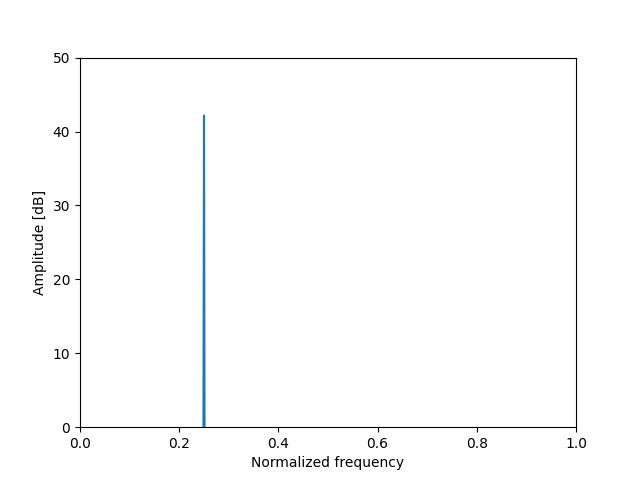
\includegraphics[width=0.20\textwidth]{wave_normal_freq8.png}
 		\vspace{-2pt}\\
 		%%%%%%%%%
 		(a) $\mathbf{X}$&\hspace{+12pt}
 		(b) $A$\\
 		%%%%%%%%%
 	\end{tabular}
 	\caption{サイン関数による画像と周波数振幅特性}
 	\label{fig:1-1-1a}
 \end{figure}
%%%%%%%%%%%%%%%%%%
%%%%%%%%%%%%%%%%%%
 \begin{figure}[H]
 	\centering
 	\begin{tabular}{cccc}
 		%%%%%%%%%
 		
\includegraphics[width=0.20\textwidth]{wave_up8.png}&\hspace{+12pt}
 		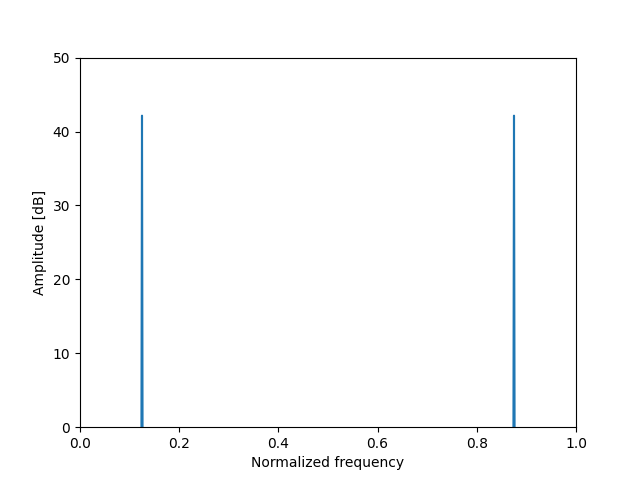
\includegraphics[width=0.20\textwidth]{wave_up_freq8.png}&\hspace{+12pt}
 		
\includegraphics[width=0.20\textwidth]{wave_down8.png}&\hspace{+12pt}
 		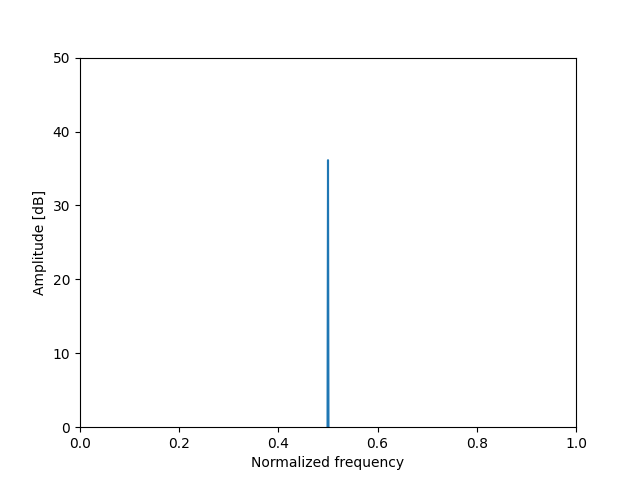
\includegraphics[width=0.20\textwidth]{wave_down_freq8.png}
 		\vspace{-2pt}\\
 		%%%%%%%%%
 		(a) $\mathbf{X}_{up}$&\hspace{+12pt}
 		(b) $A_{up}$&\hspace{+12pt}
 		(c) $\mathbf{X}_{down}$&\hspace{+12pt}
 		(d) $A_{down}$\\
 		%%%%%%%%%
 	\end{tabular}
 	\caption{アップサンプリングとダウンサンプリング後の画像と周波数振幅特性}
 	\label{fig:1-1-1b}
 \end{figure}
%%%%%%%%%%%%%%%%%%

%%%%%%%%%%%%%%%%%%
初めにピークがどこで現れるかを計算した。
$\alpha=\frac{1}{8}\pi$では周波数が $1/8$ であるため、
ピークは0.25付近に現れると予想される。また、
ダウンサンプリング後では周波数が2倍となるためピークは0.5付近
に現れると考えられる。一方、アップサンプリング後では周波数が
半分となるため0.125付近にピークが現れ、さらに0.875付近にも
ピークが現れると予想される。

実際の結果を見ると、図のピークが現れた位置と計算結果が
一致していることが分かった。また、ピーク強度は $A$ および $A_{up}$ 
では約$42\,\text{db}$であったのに対し、$A_{down}$ では約$36\,\text{db} $となった。

画像について見ると、アップサンプリング後では元画像より縞模様の周期が
長くなり、横方向に引き伸ばされたような見た目となった。一方、
ダウンサンプリング後では縞模様の周期が短くなり、元画像より細かい縞模様となった。

次に、$\alpha=\frac{1}{4}$と$\gamma=2$としたときの結果を示す。
%%%%%%%%%%%%%%%%%%
 \begin{figure}[H]
 	\centering
 	\begin{tabular}{cc}
 		%%%%%%%%%
 		
\includegraphics[width=0.20\textwidth]{wave_normal4.png}&\hspace{+12pt}
 		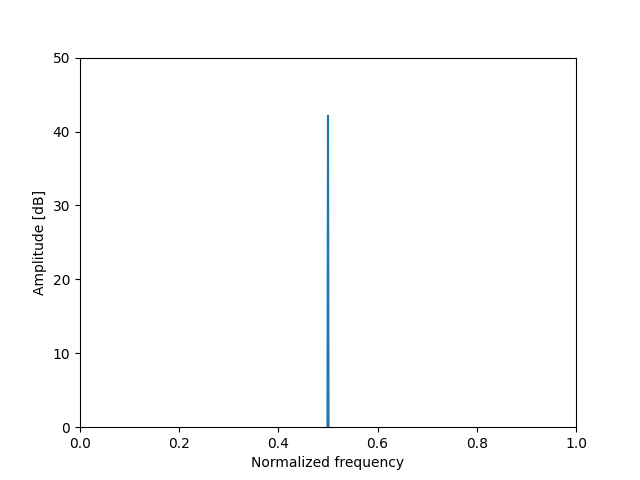
\includegraphics[width=0.20\textwidth]{wave_normal_freq4.png}
 		\vspace{-2pt}\\
 		%%%%%%%%%
 		(a) $\mathbf{X}$&\hspace{+12pt}
 		(b) $A$\\
 		%%%%%%%%%
 	\end{tabular}
 	\caption{サイン関数による画像と周波数振幅特性}
 	\label{fig:1-1-2a}
 \end{figure}
%%%%%%%%%%%%%%%%%%
%%%%%%%%%%%%%%%%%%
 \begin{figure}[H]
 	\centering
 	\begin{tabular}{cccc}
 		%%%%%%%%%
 		
\includegraphics[width=0.20\textwidth]{wave_up4.png}&\hspace{+12pt}
 		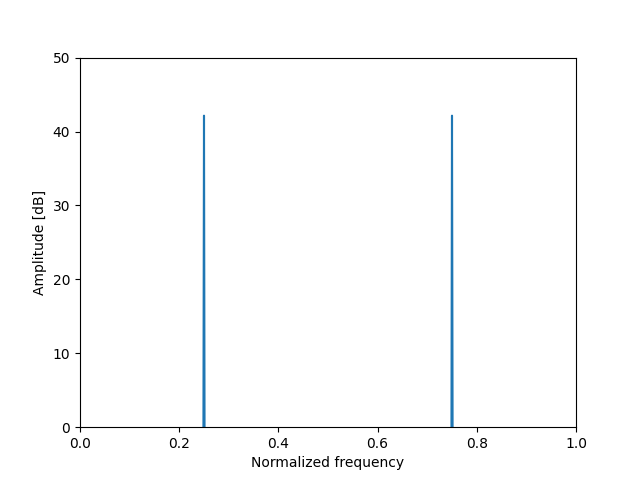
\includegraphics[width=0.20\textwidth]{wave_up_freq4.png}&\hspace{+12pt}
 		
\includegraphics[width=0.20\textwidth]{wave_down4.png}&\hspace{+12pt}
 		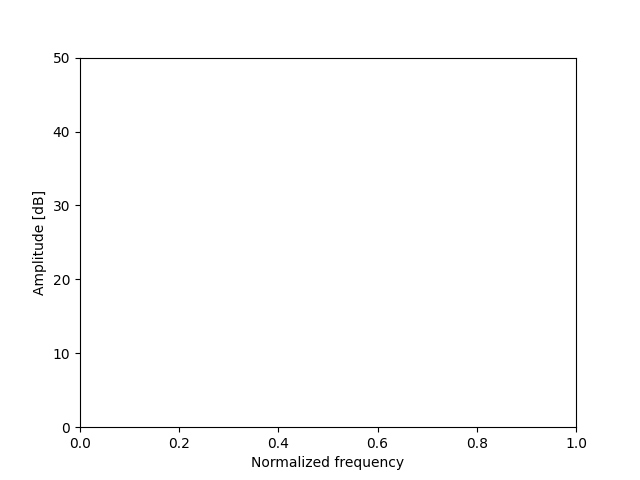
\includegraphics[width=0.20\textwidth]{wave_down_freq4.png}
 		\vspace{-2pt}\\
 		%%%%%%%%%
 		(a) $\mathbf{X}_{up}$&\hspace{+12pt}
 		(b) $A_{up}$&\hspace{+12pt}
 		(c) $\mathbf{X}_{down}$&\hspace{+12pt}
 		(d) $A_{down}$\\
 		%%%%%%%%%
 	\end{tabular}
 	\caption{アップサンプリングとダウンサンプリング後の画像と周波数振幅特性}
 	\label{fig:1-1-2b}
 \end{figure}
%%%%%%%%%%%%%%%%%%

%%%%%%%%%%%%%%%%%%

さらに、$\alpha=\frac{1}{16}$と$\gamma=2$としたときの結果を示す。
%%%%%%%%%%%%%%%%%%
 \begin{figure}[H]
 	\centering
 	\begin{tabular}{cc}
 		%%%%%%%%%
 		
\includegraphics[width=0.20\textwidth]{wave_normal16.png}&\hspace{+12pt}
 		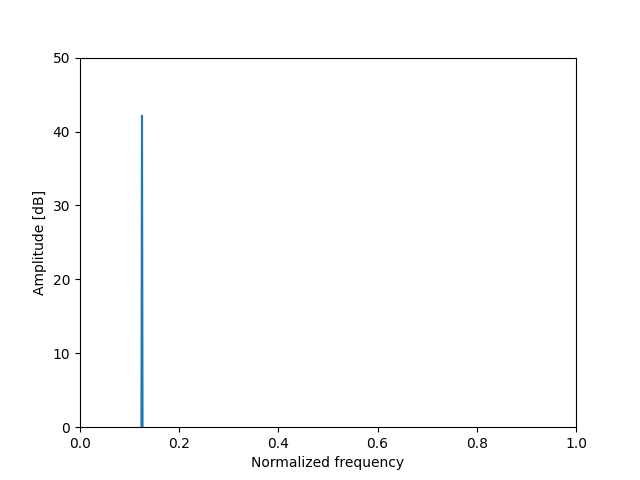
\includegraphics[width=0.20\textwidth]{wave_normal_freq16.png}
 		\vspace{-2pt}\\
 		%%%%%%%%%
 		(a) $\mathbf{X}$&\hspace{+12pt}
 		(b) $A$\\
 		%%%%%%%%%
 	\end{tabular}
 	\caption{サイン関数による画像と周波数振幅特性}
 	\label{fig:1-1-3a}
 \end{figure}
%%%%%%%%%%%%%%%%%%
%%%%%%%%%%%%%%%%%%
 \begin{figure}[H]
 	\centering
 	\begin{tabular}{cccc}
 		%%%%%%%%%
 		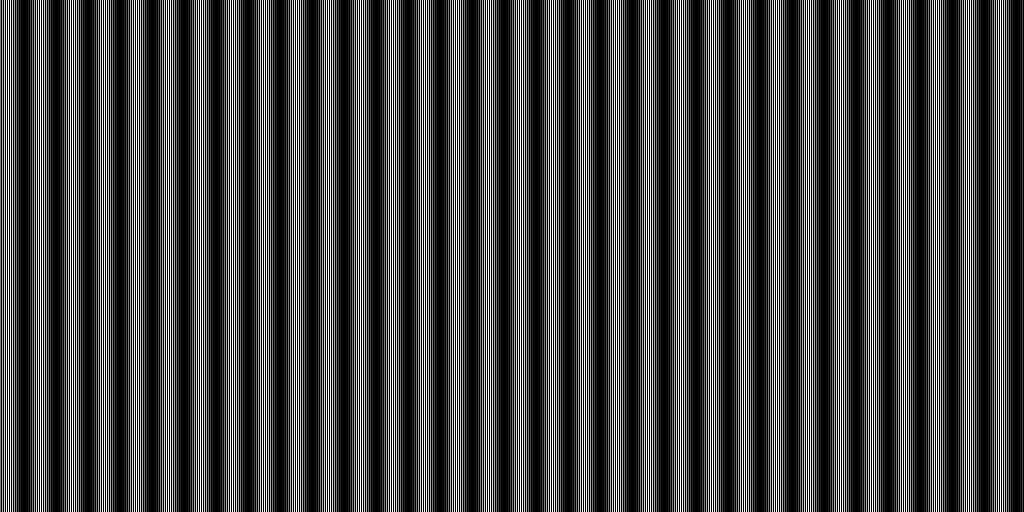
\includegraphics[width=0.20\textwidth]{wave_up16.png}&\hspace{+12pt}
 		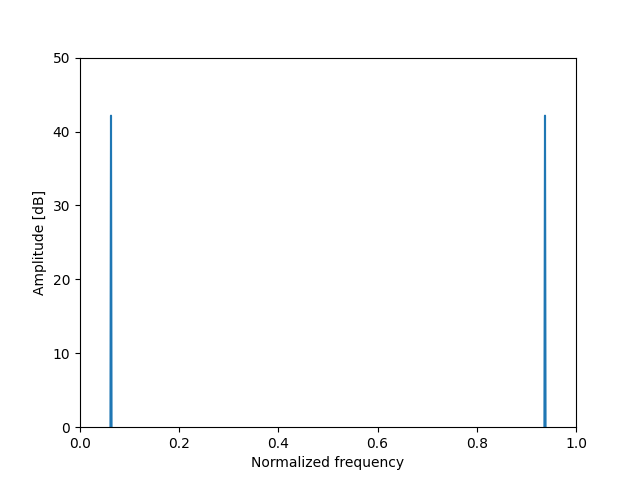
\includegraphics[width=0.20\textwidth]{wave_up_freq16.png}&\hspace{+12pt}
 		
\includegraphics[width=0.20\textwidth]{wave_down16.png}&\hspace{+12pt}
 		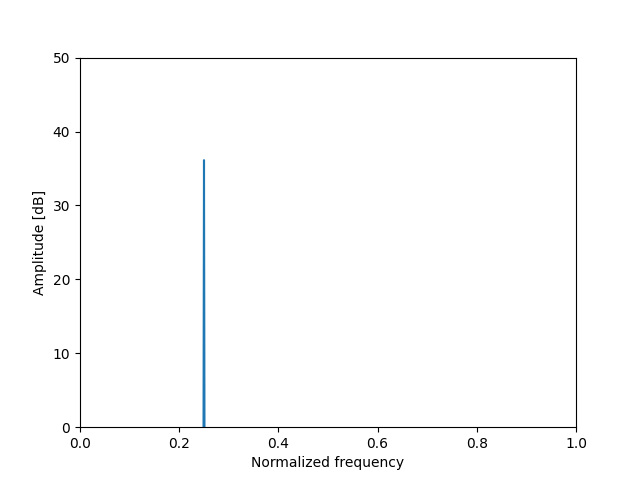
\includegraphics[width=0.20\textwidth]{wave_down_freq16.png}
 		\vspace{-2pt}\\
 		%%%%%%%%%
 		(a) $\mathbf{X}_{up}$&\hspace{+12pt}
 		(b) $A_{up}$&\hspace{+12pt}
 		(c) $\mathbf{X}_{down}$&\hspace{+12pt}
 		(d) $A_{down}$\\
 		%%%%%%%%%
 	\end{tabular}
 	\caption{アップサンプリングとダウンサンプリング後の画像と周波数振幅特性}
 	\label{fig:1-1-3b}
 \end{figure}
%%%%%%%%%%%%%%%%%%

%%%%%%%%%%%%%%%%%%


\subsection{二次元信号の周波数解析}
ここに、\ref{sec:1-2}節の結果と考察を示す。
図に、入力画像$\mathbf{X}$とそのDCTを適用した後の出力画像$\mathbf{Y}$をそれぞれ示す。

%%%%%%%%%%%%%%%%%%
 \begin{figure}[H]
 	\centering
 	\begin{tabular}{cc}
 		%%%%%%%%%
 		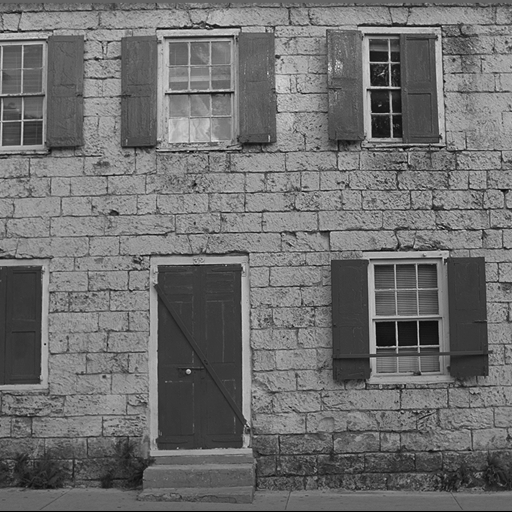
\includegraphics[width=0.20\textwidth]{kodak001.png}&\hspace{+12pt}
 		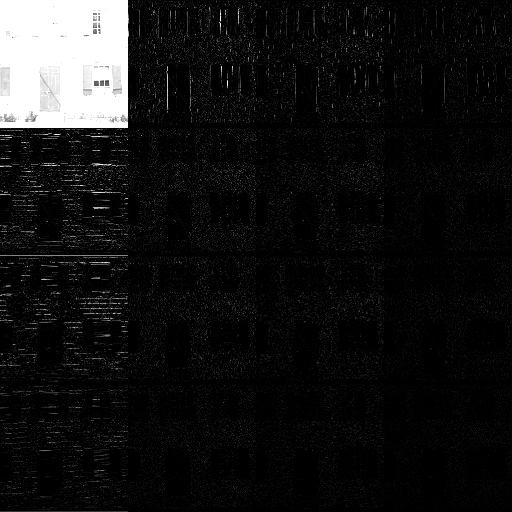
\includegraphics[width=0.20\textwidth]{kodak001_DCT.png}
 		\vspace{-2pt}\\
 		%%%%%%%%%
 		(a) $\mathbf{X}$&\hspace{+12pt}
 		(b) $\mathbf{Y}$\\
 		%%%%%%%%%
 	\end{tabular}
 	\caption{入力画像とDCT後の出力画像(画像:kodak001)}
 	\label{fig:1-2-1}
 \end{figure}
%%%%%%%%%%%%%%%%%%

%%%%%%%%%%%%%%%%%%

まず左上のブロックが白くなっており、画像の情報の多くが
低周波成分に集中していることが分かる。
また、縦方向および横方向の周波数成分のブロックでは
、壁とドアまたは窓との境界部分に白い線が現れていた。
これは境界付近で画素値が変化しているためである。
一方で、これらの白い線は低周波領域で強く現れ、高周波領域へ移るにつれて徐々に薄くなっていた。
よって、これらの境界は比較的なだらかな変化として表現されており、高周波成分の寄与は小さいことが分かる。

%%%%%%%%%%%%%%%%%%
 \begin{figure}[H]
 	\centering
 	\begin{tabular}{cc}
 		%%%%%%%%%
 		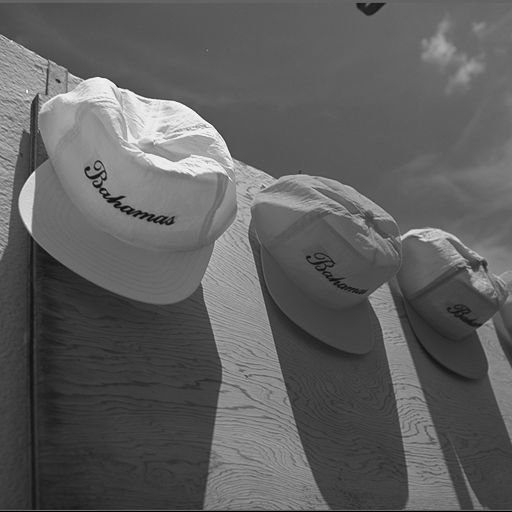
\includegraphics[width=0.20\textwidth]{kodak002.png}&\hspace{+12pt}
 		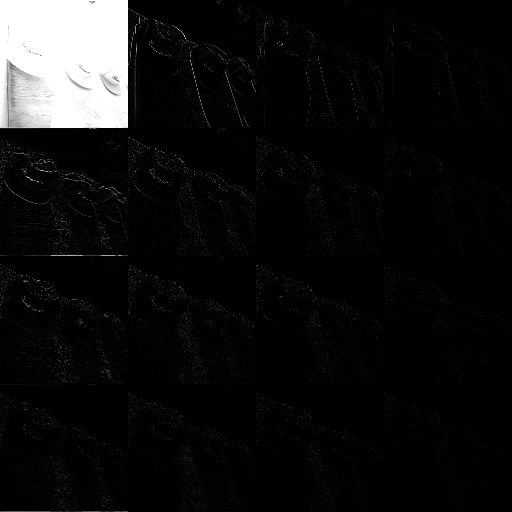
\includegraphics[width=0.20\textwidth]{kodak002_DCT.png}
 		\vspace{-2pt}\\
 		%%%%%%%%%
 		(a) $\mathbf{X}$&\hspace{+12pt}
 		(b) $\mathbf{Y}$\\
 		%%%%%%%%%
 	\end{tabular}
 	\caption{入力画像とDCT後の出力画像(画像:kodak002)}
 	\label{fig:1-2-2}
 \end{figure}
%%%%%%%%%%%%%%%%%%

%%%%%%%%%%%%%%%%%%


この画像も同様に左上のブロックが白くなっており、
画像の情報の多くが低周波成分に集中していることが分かる。
また、帽子とその影との境界や影と壁との境界や壁と空との境界部分に白い線が観察された。
そして、これらの白い線は低周波領域で強く現れ、高周波領域へ移るにつれて徐々に薄くなっていた。
よって、この画像の輪郭情報も主に低周波成分に含まれており、高周波成分の寄与は比較的小さいことが分かる。
また，前画像と比較すると、斜め右下方向のサブバンドにも比較的強い成分が見られた。
これは、本画像には帽子や影の輪郭など曲線的な構造が多く含まれており、
建物画像に多く見られた水平・垂直方向の直線的な構造だけでは表現できないためと考えられる。
そのため、縦方向成分と横方向成分の両方を含む周波数成分の寄与が大きくなったと考えられる。

%%%%%%%%%%%%%%%%%%
 \begin{figure}[H]
 	\centering
 	\begin{tabular}{cc}
 		%%%%%%%%%
 		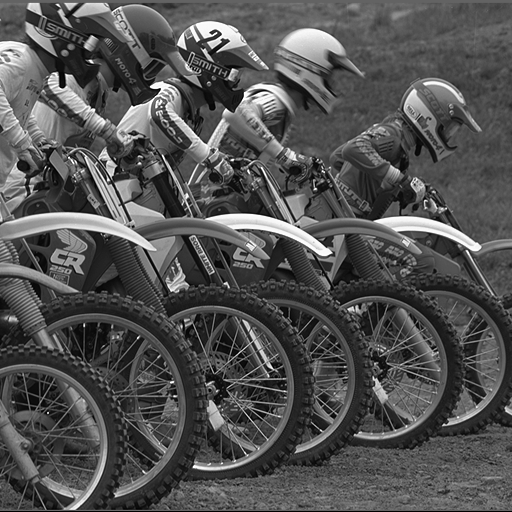
\includegraphics[width=0.20\textwidth]{kodak003.png}&\hspace{+12pt}
 		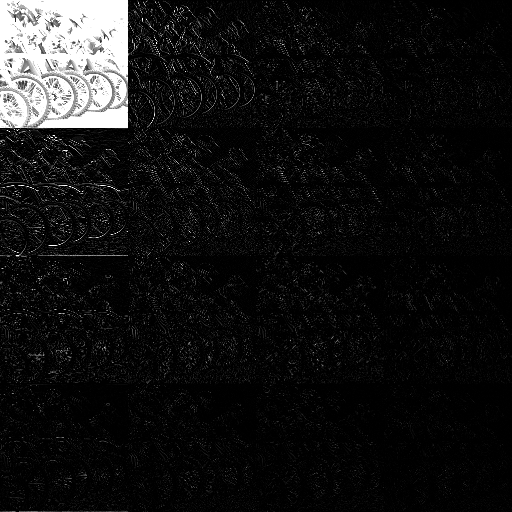
\includegraphics[width=0.20\textwidth]{kodak003_DCT.png}
 		\vspace{-2pt}\\
 		%%%%%%%%%
 		(a) $\mathbf{X}$&\hspace{+12pt}
 		(b) $\mathbf{Y}$\\
 		%%%%%%%%%
 	\end{tabular}
 	\caption{入力画像とDCT後の出力画像(画像:kodak003)}
 	\label{fig:1-2-3}
 \end{figure}
%%%%%%%%%%%%%%%%%%

%%%%%%%%%%%%%%%%%%
この画像も同様に左上のブロックが白くなっており、画像の情報の多くが低周波成分に集中していることが分かる。
また、バイクやライダーの輪郭、タイヤのスポーク部分などに対応する白い線が観察された。
そして、高周波領域へ移るにつれて全体的な強度は小さくなっている。
これまでの画像と比較すると、右側および下側のサブバンドにも比較的強い成分が見られた。
これは、タイヤのスポークや車体の細かな部品など、高周波成分を多く含む構造が存在するためと考えられる。


\subsection{画像の逆変換}


ここに、\ref{sec:1-3}節の結果と考察を示す。
図に、入力画像$\mathbf{X}$とそれをDCTした後に逆変換を行った出力画像$\mathbf{Z}$をそれぞれ示す。


%%%%%%%%%%%%%%%%%%
\begin{figure}[H]
	\centering
	\begin{tabular}{cc}
		%%%%%%%%%
		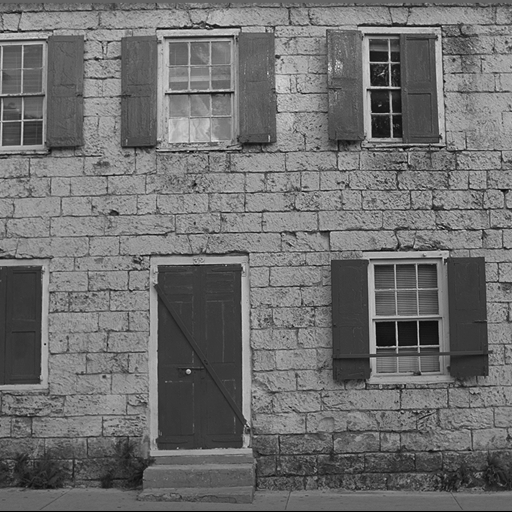
\includegraphics[width=0.20\textwidth]{kodak001.png}&\hspace{+12pt}
		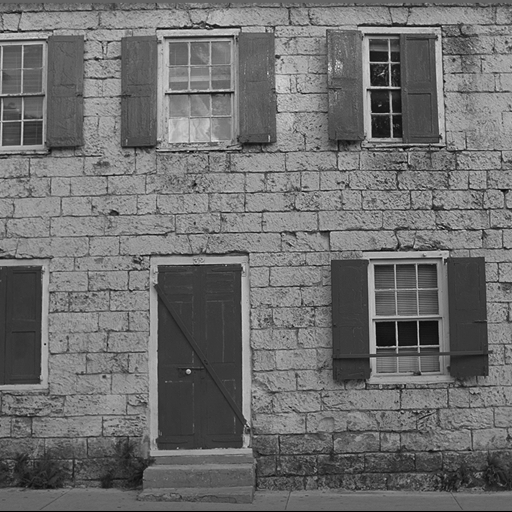
\includegraphics[width=0.20\textwidth]{kodak001_inverse.png}
		\vspace{-2pt}\\
		%%%%%%%%%
		(a) $\mathbf{X}$&\hspace{+12pt}
		(b) $\mathbf{Z}$\\
		%%%%%%%%%
	\end{tabular}
	\caption{入力画像とDCTの逆変換後の出力画像(画像:kodak001)}
	\label{fig:1-3-1}
\end{figure}
%%%%%%%%%%%%%%%%%%
%%%%%%%%%%%%%%%%%%
\begin{figure}[H]
	\centering
	\begin{tabular}{cc}
		%%%%%%%%%
		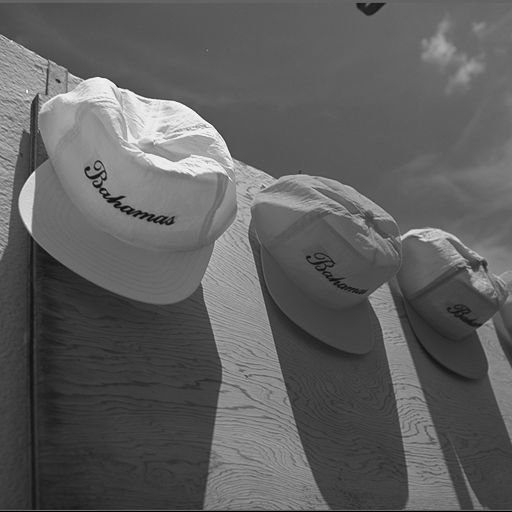
\includegraphics[width=0.20\textwidth]{kodak002.png}&\hspace{+12pt}
		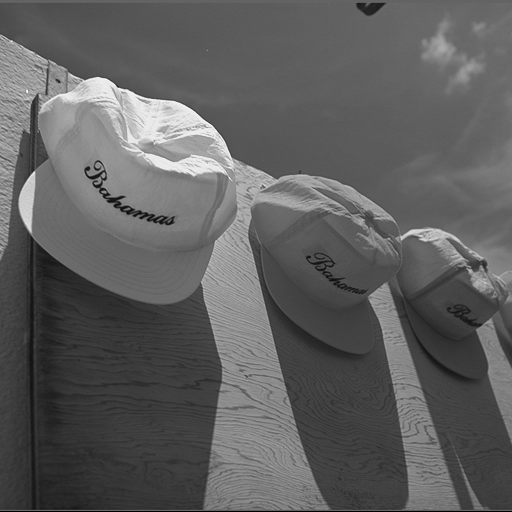
\includegraphics[width=0.20\textwidth]{kodak002_inverse.png}
		\vspace{-2pt}\\
		%%%%%%%%%
		(a) $\mathbf{X}$&\hspace{+12pt}
		(b) $\mathbf{Z}$\\
		%%%%%%%%%
	\end{tabular}
	\caption{入力画像とDCTの逆変換後の出力画像(画像:kodak002)}
	\label{fig:1-3-2}
\end{figure}
%%%%%%%%%%%%%%%%%%
%%%%%%%%%%%%%%%%%%
\begin{figure}[H]
	\centering
	\begin{tabular}{cc}
		%%%%%%%%%
		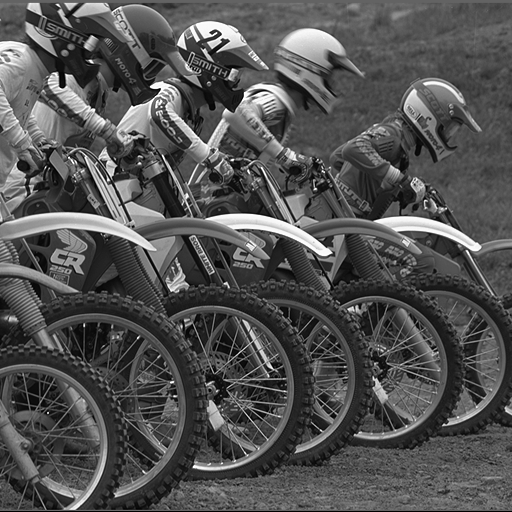
\includegraphics[width=0.20\textwidth]{kodak003.png}&\hspace{+12pt}
		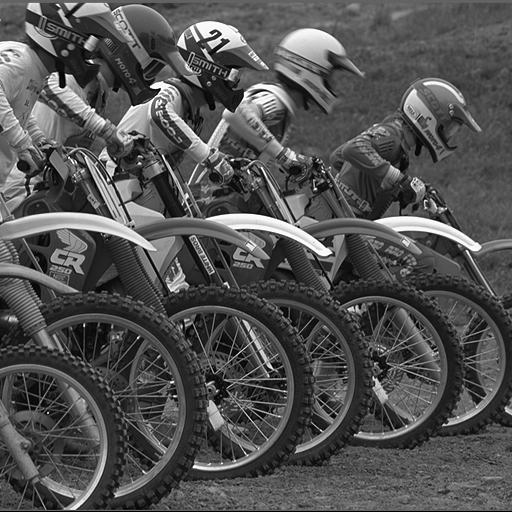
\includegraphics[width=0.20\textwidth]{kodak003_inverse.png}
		\vspace{-2pt}\\
		%%%%%%%%%
		(a) $\mathbf{X}$&\hspace{+12pt}
		(b) $\mathbf{Z}$\\
		%%%%%%%%%
	\end{tabular}
	\caption{入力画像とDCTの逆変換後の出力画像(画像:kodak003)}
	\label{fig:1-3-3}
\end{figure}
%%%%%%%%%%%%%%%%%%
逆変換後の画像$\mathbf{Z}$は、入力画像$\mathbf{X}$と見た目にはほぼ一致していた。
また、誤差$L$は1枚目で$1.78\times10^{-9}$，
2枚目で$1.14\times10^{-9}$，
3枚目で$1.65\times10^{-9}$となった。
いずれも非常に小さい値であるため、DCT変換後に逆DCTを行うことで、
元画像をほぼ完全に復元できたことが分かる。
完全に0にならなかった理由は、計算機上で小数を扱う際の丸め誤差によるものと考えられる。

\subsection{ガウシアンフィルタによる画像のぼかし}
ここに、\ref{sec:2-1}節の結果と考察を示す。
図に、$k=7$と$\sigma=4$におけるガウシアンフィルタの周波数振幅特性のグラフ$G$と入力画像$\mathbf{X}$、出力画像$\mathbf{Y}$をそれぞれ示す。

%%%%%%%%%%%%%%%%%%
\begin{figure}[H]
	\centering
	\begin{tabular}{ccc}
		%%%%%%%%%
		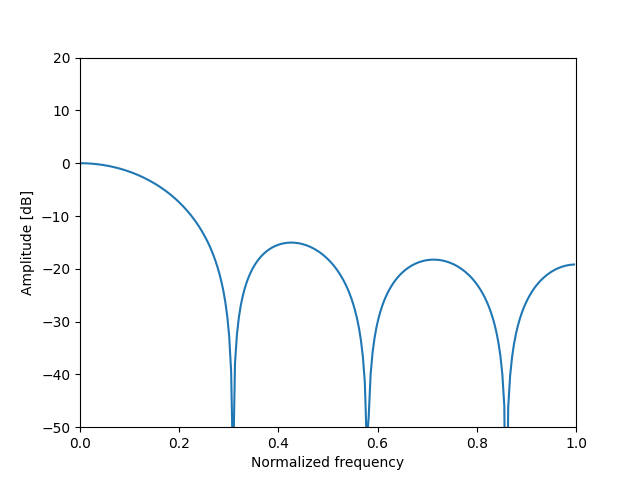
\includegraphics[width=0.20\textwidth]{freq_gauss1.png}&\hspace{+12pt}
		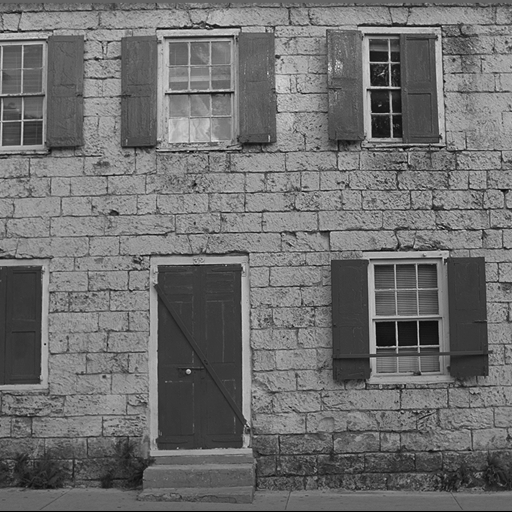
\includegraphics[width=0.20\textwidth]{kodak001.png}&\hspace{+12pt}
		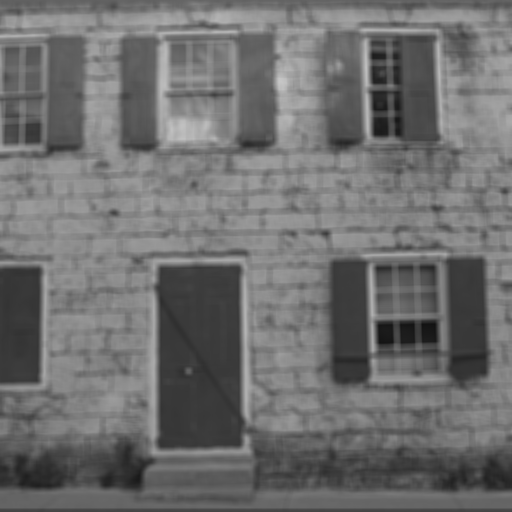
\includegraphics[width=0.20\textwidth]{kodak001_blur1.png}
		\vspace{-2pt}\\
		%%%%%%%%%
		(a) $G$&\hspace{+12pt}
		(b) $\mathbf{X}$&\hspace{+12pt}
		(c) $\mathbf{Y}$\\
		%%%%%%%%%
	\end{tabular}
	\caption{ガウシアンフィルタの周波数振幅特性と画像に適用した場合の入力と出力画像($k=7$,$\sigma=4$)}
	\label{fig:2-1-1}
\end{figure}
%%%%%%%%%%%%%%%%%%

周波数振幅特性より、0～0.2付近の周波数帯では振幅がほぼ0 dBに保たれており、
この周波数帯の成分はほとんど減衰せずに通過していることが分かる。一方、
それより高い周波数帯では、急激な谷が現れる箇所を除いて振幅が全体的に低下している。
出力画像を見ると、入力画像と比較して全体的にうっすらとぼやけていることが確認できる。
これは、4.2の実験結果からこの画像の主な成分が低周波領域に分布しているため、
高周波成分のみが抑制されても画像全体の変化が小さいためであると考えられる。

次に、$k=3$,$\sigma=1$と$k=15$,$\sigma=8$と$k=7$,$\sigma=13$におけるガウシアンフィルタの周波数振幅特性のグラフ$G$と入力画像$\mathbf{X}$、出力画像$\mathbf{Y}$をそれぞれ示す。


%%%%%%%%%%%%%%%%%%

%%%%%%%%%%%%%%%%%%
\begin{figure}[H]
	\centering
	\begin{tabular}{ccc}
		%%%%%%%%%
		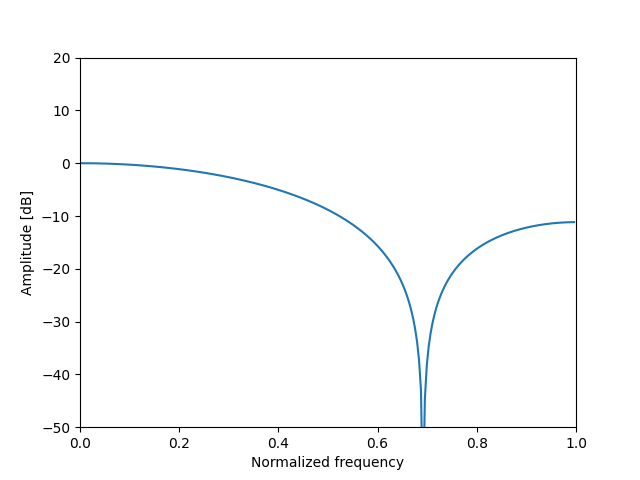
\includegraphics[width=0.20\textwidth]{freq_gaussk3s1.png}&\hspace{+12pt}
		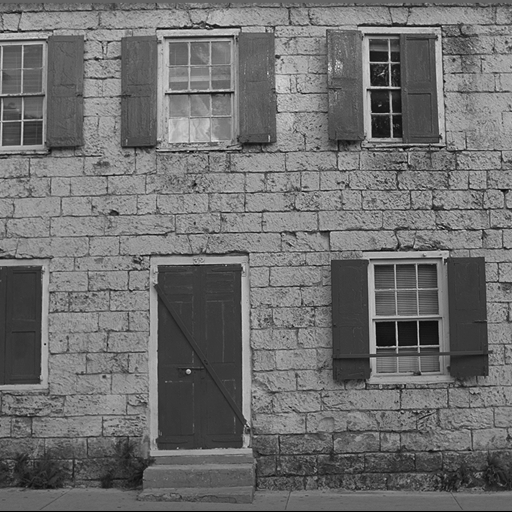
\includegraphics[width=0.20\textwidth]{kodak001.png}&\hspace{+12pt}
		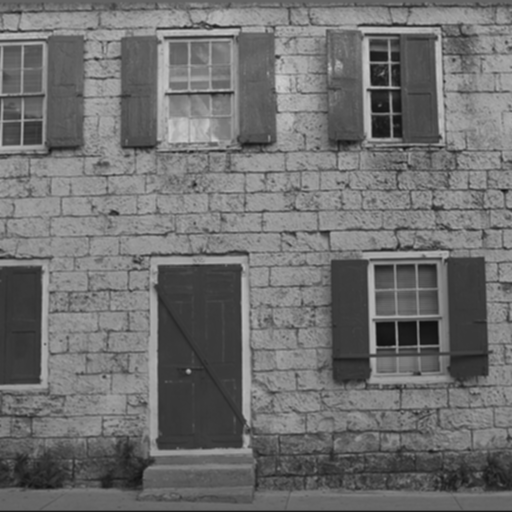
\includegraphics[width=0.20\textwidth]{kodak001_blurk3s1.png}
		\vspace{-2pt}\\
		%%%%%%%%%
		(a) $G$&\hspace{+12pt}
		(b) $\mathbf{X}$&\hspace{+12pt}
		(c) $\mathbf{Y}$\\
		%%%%%%%%%
	\end{tabular}
	\caption{ガウシアンフィルタの周波数振幅特性と画像に適用した場合の入力と出力画像($k=3$,$\sigma=1$)}
	\label{fig:2-1-2}
\end{figure}
%%%%%%%%%%%%%%%%%%

%%%%%%%%%%%%%%%%%%

%%%%%%%%%%%%%%%%%%
\begin{figure}[H]
	\centering
	\begin{tabular}{ccc}
		%%%%%%%%%
		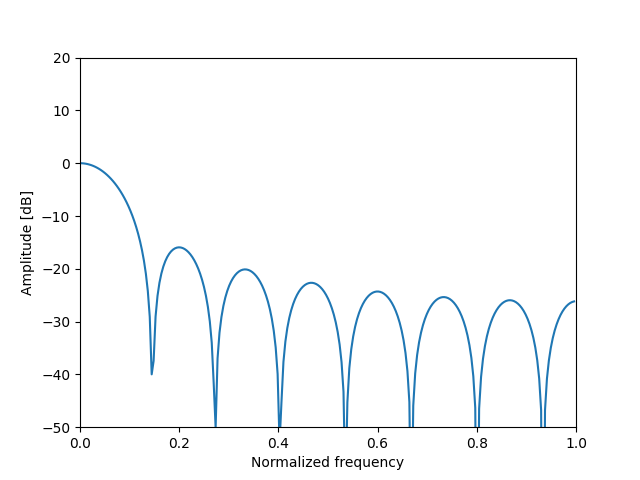
\includegraphics[width=0.20\textwidth]{freq_gaussk15s8.png}&\hspace{+12pt}
		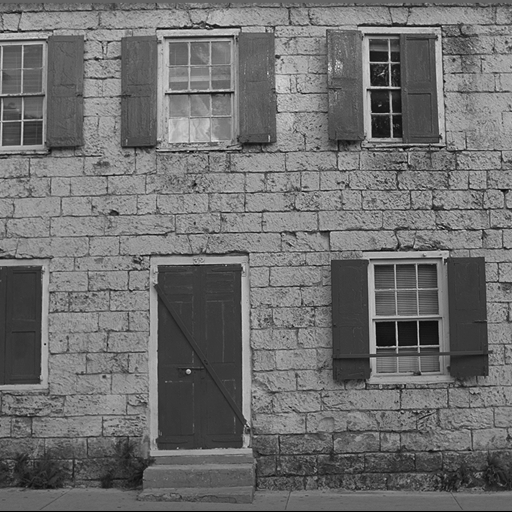
\includegraphics[width=0.20\textwidth]{kodak001.png}&\hspace{+12pt}
		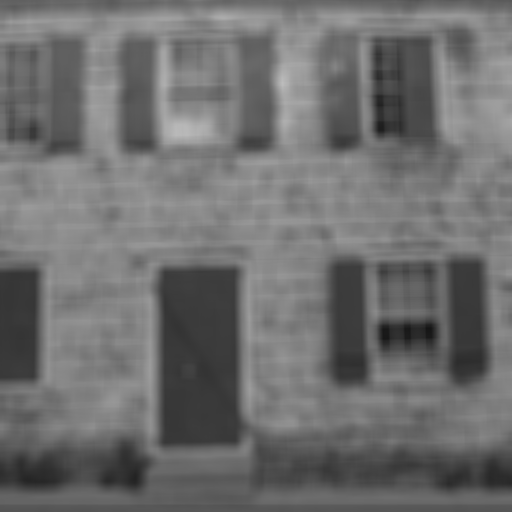
\includegraphics[width=0.20\textwidth]{kodak001_blurk15s8.png}
		\vspace{-2pt}\\
		%%%%%%%%%
		(a) $G$&\hspace{+12pt}
		(b) $\mathbf{X}$&\hspace{+12pt}
		(c) $\mathbf{Y}$\\
		%%%%%%%%%
	\end{tabular}
	\caption{ガウシアンフィルタの周波数振幅特性と画像に適用した場合の入力と出力画像($k=15$,$\sigma=8$)}
	\label{fig:2-1-3}
\end{figure}
%%%%%%%%%%%%%%%%%%

%%%%%%%%%%%%%%%%%%

%%%%%%%%%%%%%%%%%%
\begin{figure}[H]
	\centering
	\begin{tabular}{ccc}
		%%%%%%%%%
		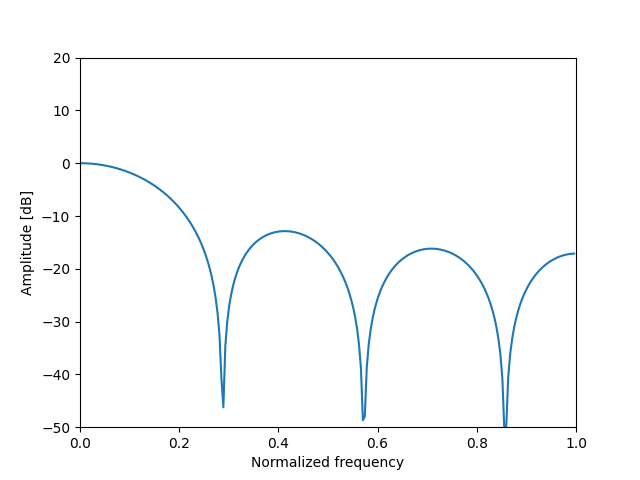
\includegraphics[width=0.20\textwidth]{freq_gaussk7s13.png}&\hspace{+12pt}
		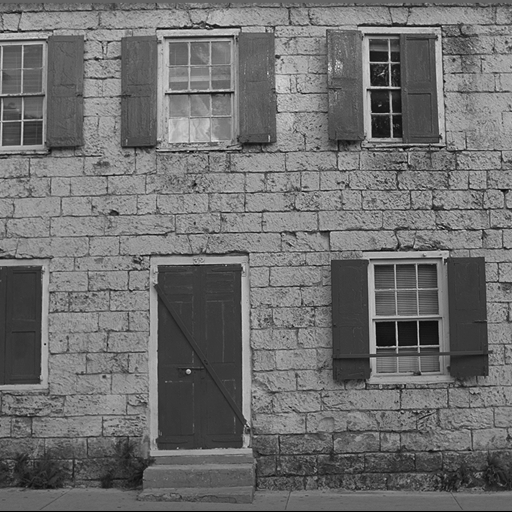
\includegraphics[width=0.20\textwidth]{kodak001.png}&\hspace{+12pt}
		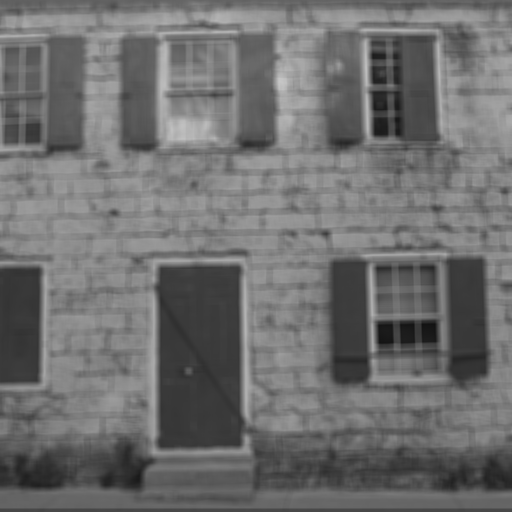
\includegraphics[width=0.20\textwidth]{kodak001_blurk7s13.png}
		\vspace{-2pt}\\
		%%%%%%%%%
		(a) $G$&\hspace{+12pt}
		(b) $\mathbf{X}$&\hspace{+12pt}
		(c) $\mathbf{Y}$\\
		%%%%%%%%%
	\end{tabular}
	\caption{ガウシアンフィルタの周波数振幅特性と画像に適用した場合の入力と出力画像($k=7$,$\sigma=13$)}
	\label{fig:2-1-4}
\end{figure}
%%%%%%%%%%%%%%%%%%

%%%%%%%%%%%%%%%%%%
$k=3,\sigma=1$の場合は高周波成分が比較的保持されており、
出力画像でも石壁や窓枠などの細かな模様が残っていた。一方、
$k=15,\sigma=8$の場合は高周波成分がより抑制され、
出力画像では細部が平滑化されて強いぼかし効果が確認できた。
また、$k=7,\sigma=13$の場合は、$k=7,\sigma=4$の場合と比較して
周波数振幅特性および出力画像に大きな違いは見られなかった。これは、
フィルタ長が固定されているため、$\sigma$を大きくしても平滑化効果の変化が小さかったためと考えられる。以上より，今回の実験では$\sigma$よりも$k$の変化の方が出力画像に与える影響が大きいことが分かった。

\subsection{画像のノイズとその除去}
ここに、\ref{sec:2-2}節の結果と考察を示す。
図に、$k=5$と$\sigma=3$、$\sigma_n=15$における原画像$\mathbf{X}$とそのノイズあり画像$\mathbf{Y}$、ガウシアンフィルタによる平滑化後の出力画像$\mathbf{Z}$をそれぞれ示す。

%%%%%%%%%%%%%%%%%%
\begin{figure}[H]
	\centering
	\begin{tabular}{ccc}
		%%%%%%%%%
		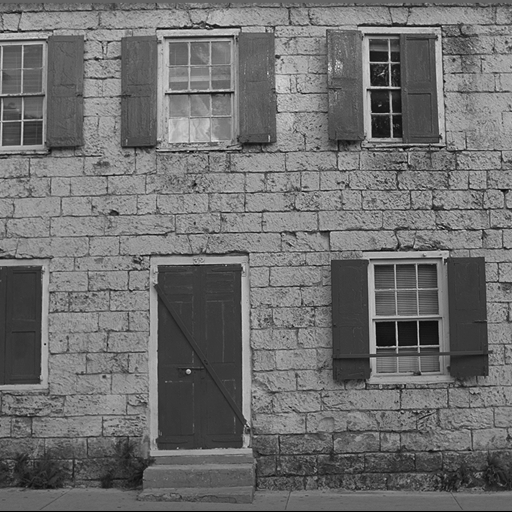
\includegraphics[width=0.20\textwidth]{kodak001.png}&\hspace{+12pt}
		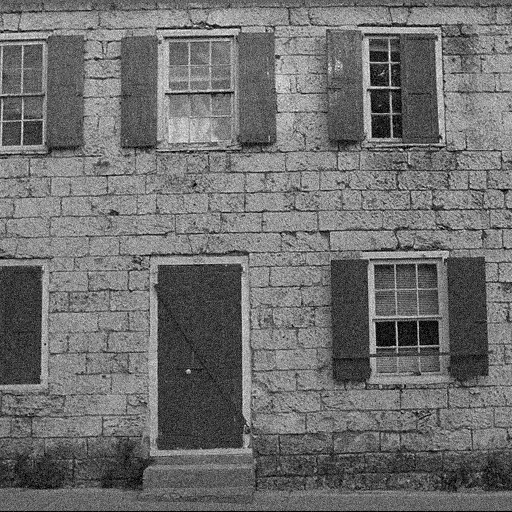
\includegraphics[width=0.20\textwidth]{kodak001_noisys15k5s3}&\hspace{+12pt}
		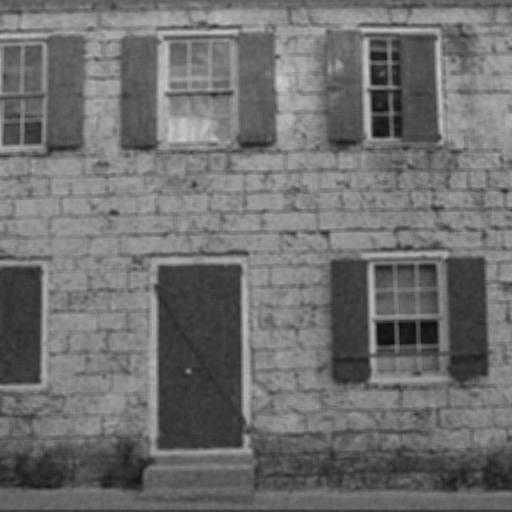
\includegraphics[width=0.20\textwidth]{kodak001_denoiseds15k5s3.png}
		\vspace{-2pt}\\
		%%%%%%%%%
		(a) $\mathbf{X}$&\hspace{+12pt}
		(b) $\mathbf{Y}$&\hspace{+12pt}
		(c) $\mathbf{Z}$\\
		%%%%%%%%%
	\end{tabular}
	\caption{原画像とノイズあり画像、ノイズ除去後の出力画像($k=5$,$\sigma=3$,$\sigma_n=15$)}
	\label{fig:2-3-1}
\end{figure}
%%%%%%%%%%%%%%%%%%

%%%%%%%%%%%%%%%%%%
入力画像に標準偏差15のガウスノイズを加えた結果、画像全体に細かな粒状のノイズが発生した。
これに対して、サイズ5×5、標準偏差3のガウシアンフィルタを適用すると、
画像は全体的に平滑化され、ぼやけた見た目となった。
一方で、ノイズの強さが比較的小さいため、ノイズ除去効果は視覚的に分かりにくかった。

次に$k=3$,$\sigma=1$、$\sigma_n=25$と$k=3$、$\sigma=1$、$\sigma_n=35$の場合の結果を示す。


%%%%%%%%%%%%%%%%%%
\begin{figure}[H]
	\centering
	\begin{tabular}{ccc}
		%%%%%%%%%
		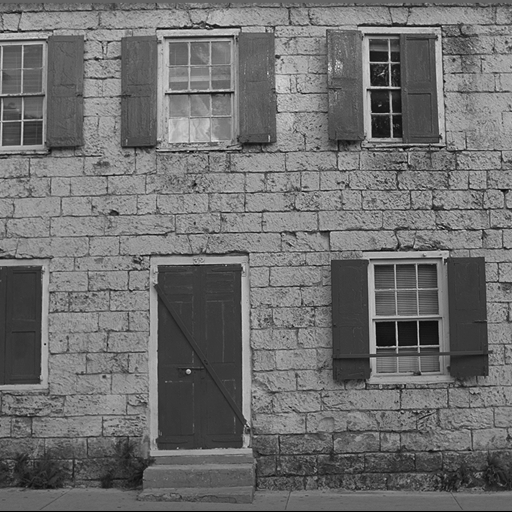
\includegraphics[width=0.20\textwidth]{kodak001.png}&\hspace{+12pt}
		\includegraphics[width=0.20\textwidth]{kodak001_noisys25k3s1}&\hspace{+12pt}
		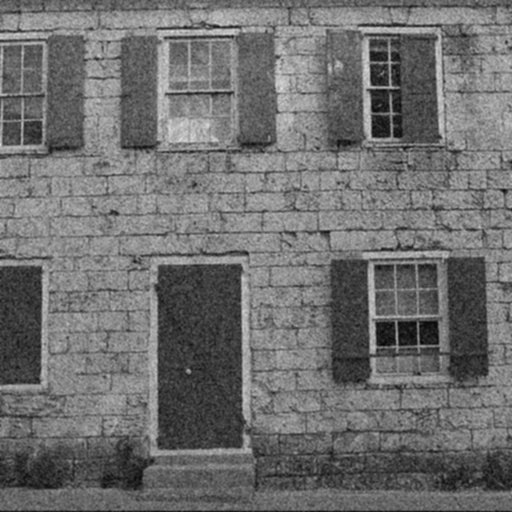
\includegraphics[width=0.20\textwidth]{kodak001_denoiseds25k3s1.png}
		\vspace{-2pt}\\
		%%%%%%%%%
		(a) $\mathbf{X}$&\hspace{+12pt}
		(b) $\mathbf{Y}$&\hspace{+12pt}
		(c) $\mathbf{Z}$\\
		%%%%%%%%%
	\end{tabular}
	\caption{原画像とノイズあり画像、ノイズ除去後の出力画像($k=3$,$\sigma=1$,$\sigma_n=25$)}
	\label{fig:2-3-2}
\end{figure}
%%%%%%%%%%%%%%%%%%

%%%%%%%%%%%%%%%%%%

%%%%%%%%%%%%%%%%%%
\begin{figure}[H]
	\centering
	\begin{tabular}{ccc}
		%%%%%%%%%
		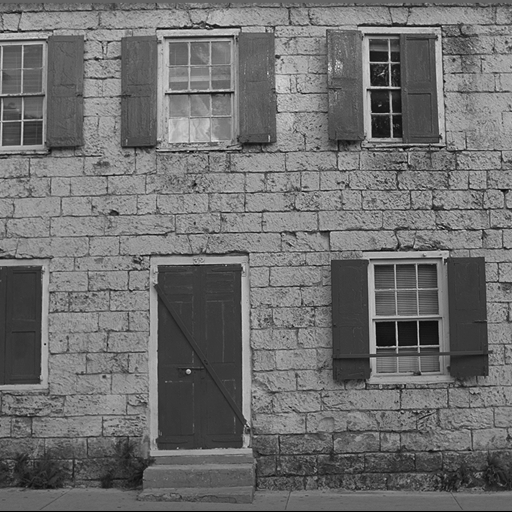
\includegraphics[width=0.20\textwidth]{kodak001.png}&\hspace{+12pt}
		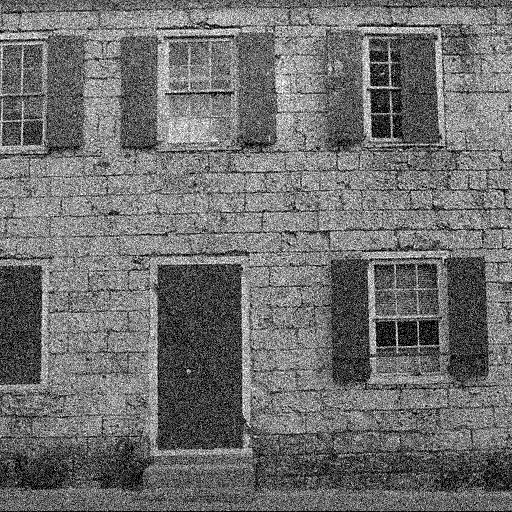
\includegraphics[width=0.20\textwidth]{kodak001_noisys35k3s1}&\hspace{+12pt}
		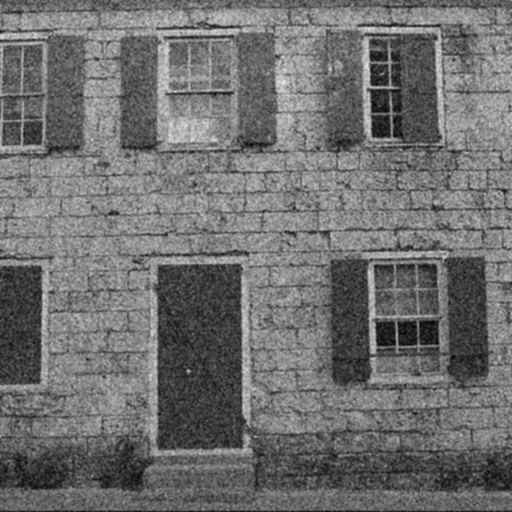
\includegraphics[width=0.20\textwidth]{kodak001_denoiseds35k3s1.png}
		\vspace{-2pt}\\
		%%%%%%%%%
		(a) $\mathbf{X}$&\hspace{+12pt}
		(b) $\mathbf{Y}$&\hspace{+12pt}
		(c) $\mathbf{Z}$\\
		%%%%%%%%%
	\end{tabular}
	\caption{原画像とノイズあり画像、ノイズ除去後の出力画像($k=3$,$\sigma=1$,$\sigma_n=35$)}
	\label{fig:2-3-3}
\end{figure}
%%%%%%%%%%%%%%%%%%

%%%%%%%%%%%%%%%%%%
サイズ3×3、標準偏差1のガウシアンフィルタを適用した結果、
ノイズはわずかに低減されたものの、その変化は大きくなかった。
入力画像に標準偏差35のガウスノイズを加えた結果、図\ref{fig:2-3-2}よりも
強い粒状ノイズが発生した。これに対して、サイズ3×3、標準偏差1のガウシアンフィルタを適用すると、
ノイズはある程度低減されたことが確認できた。しかし、平滑化の強さが小さいためノイズを完全に除去する
ことはできず、一部のノイズは残存した。

\subsection{ソーベルフィルタによる画像のエッジ検出}
ここに、\ref{sec:2-3}節の結果と考察を示す。
図に、ソーベルフィルタの周波数振幅特性$S$と入力画像$\mathbf{X}$、$\mathbf{X}$に縦と横方向のソーベルフィルタを適用した出力画像$\mathbf{S}_v$と$\mathbf{S}_h$をそれぞれ示す。

%%%%%%%%%%%%%%%%%%
\begin{figure}[H]
	\centering
	\begin{tabular}{cccc}
		%%%%%%%%%
		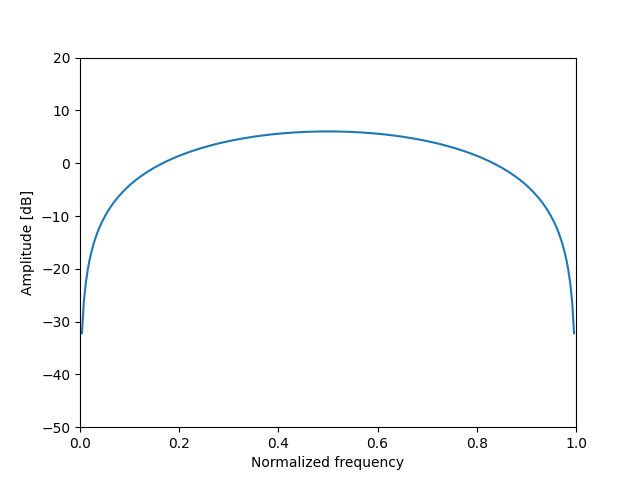
\includegraphics[width=0.20\textwidth]{freq_sobel1.png}&\hspace{+12pt}
		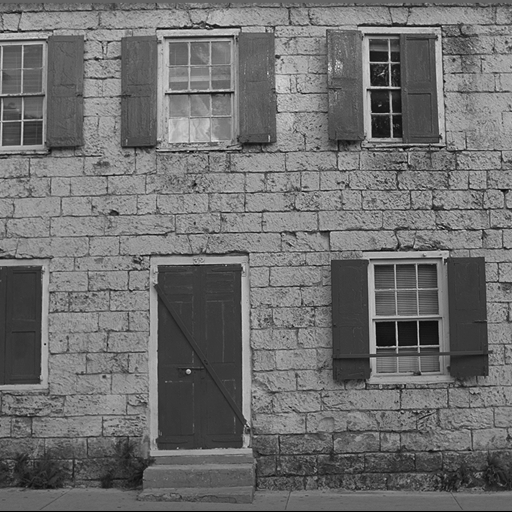
\includegraphics[width=0.20\textwidth]{kodak001.png}&\hspace{+12pt}
		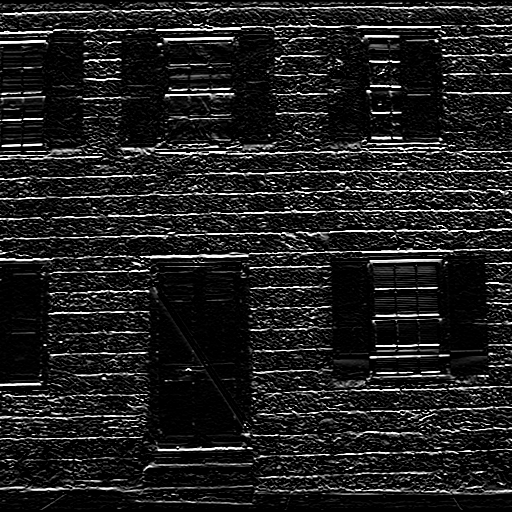
\includegraphics[width=0.20\textwidth]{kodak001_sobel_v1.png}&\hspace{+12pt}
		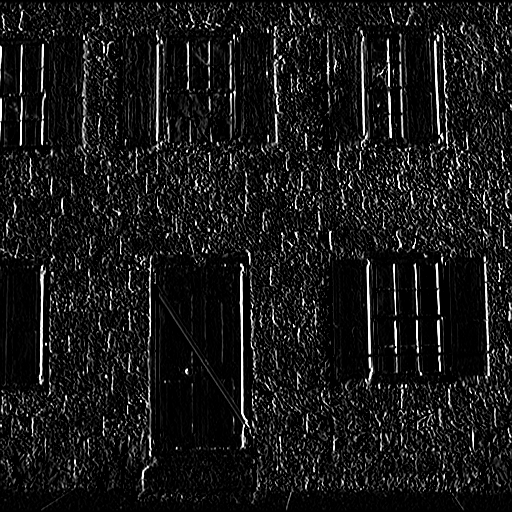
\includegraphics[width=0.20\textwidth]{kodak001_sobel_h1.png}
		\vspace{-2pt}\\
		%%%%%%%%%
		(a) $S$&\hspace{+12pt}
		(b) $\mathbf{X}$&\hspace{+12pt}
		(c) $\mathbf{S}_{v}$&\hspace{+12pt}
		(d) $\mathbf{S}_{h}$\\
		%%%%%%%%%
	\end{tabular}
	\caption{ソーベルフィルタの周波数振幅特性と画像に適用した場合の入力と出力画像}
	\label{fig:2-2-1}
\end{figure}
%%%%%%%%%%%%%%%%%%

%%%%%%%%%%%%%%%%%%
\begin{figure}[H]
	\centering
	\begin{tabular}{cccc}
		%%%%%%%%%
		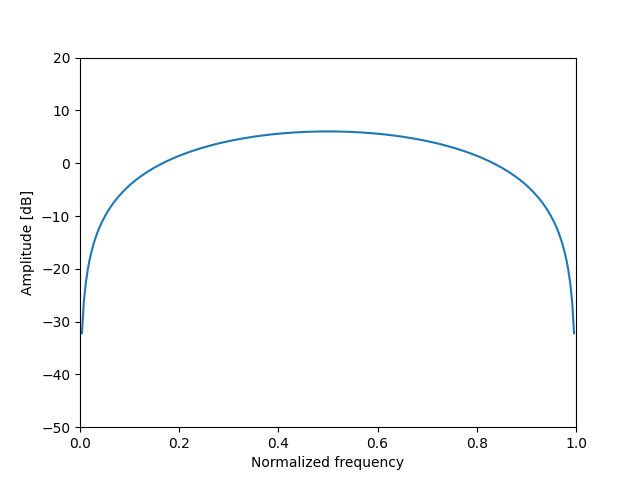
\includegraphics[width=0.20\textwidth]{freq_sobel2.png}&\hspace{+12pt}
		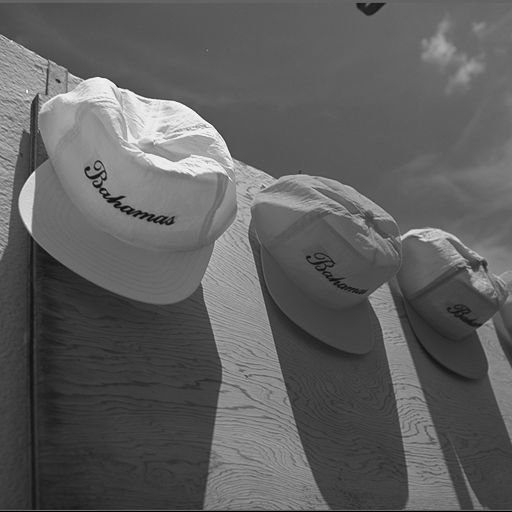
\includegraphics[width=0.20\textwidth]{kodak002.png}&\hspace{+12pt}
		\includegraphics[width=0.20\textwidth]{kodak002_sobel_v1.png}&\hspace{+12pt}
		\includegraphics[width=0.20\textwidth]{kodak002_sobel_h1.png}
		\vspace{-2pt}\\
		%%%%%%%%%
		(a) $S$&\hspace{+12pt}
		(b) $\mathbf{X}$&\hspace{+12pt}
		(c) $\mathbf{S}_{v}$&\hspace{+12pt}
		(d) $\mathbf{S}_{h}$\\
		%%%%%%%%%
	\end{tabular}
	\caption{ソーベルフィルタの周波数振幅特性と画像に適用した場合の入力と出力画像}
	\label{fig:2-2-2}
\end{figure}
%%%%%%%%%%%%%%%%%%

%%%%%%%%%%%%%%%%%%
\begin{figure}[H]
	\centering
	\begin{tabular}{cccc}
		%%%%%%%%%
		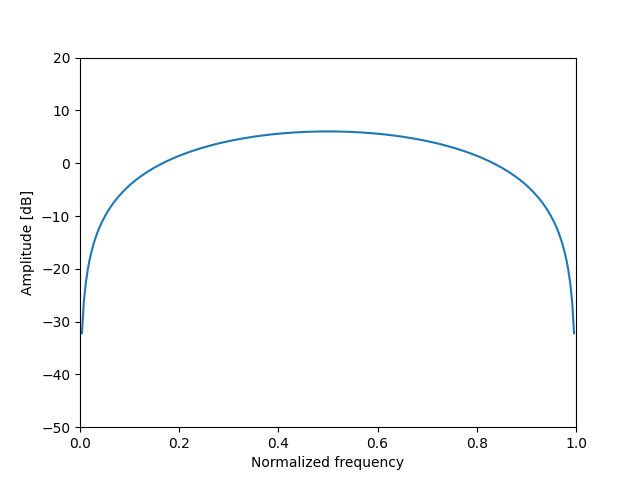
\includegraphics[width=0.20\textwidth]{freq_sobel3.png}&\hspace{+12pt}
		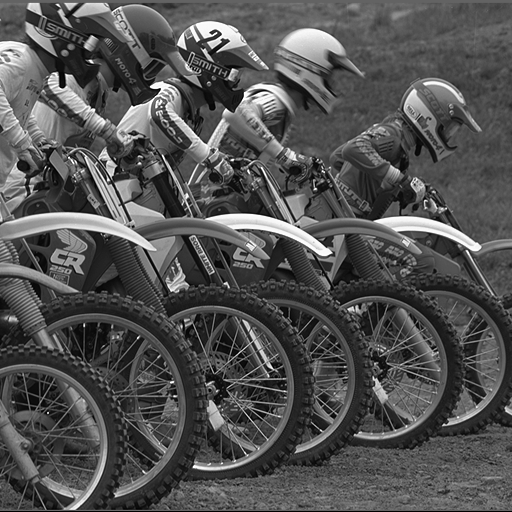
\includegraphics[width=0.20\textwidth]{kodak003.png}&\hspace{+12pt}
		\includegraphics[width=0.20\textwidth]{kodak003_sobel_v1.png}&\hspace{+12pt}
		\includegraphics[width=0.20\textwidth]{kodak003_sobel_h1.png}
		\vspace{-2pt}\\
		%%%%%%%%%
		(a) $S$&\hspace{+12pt}
		(b) $\mathbf{X}$&\hspace{+12pt}
		(c) $\mathbf{S}_{v}$&\hspace{+12pt}
		(d) $\mathbf{S}_{h}$\\
		%%%%%%%%%
	\end{tabular}
	\caption{ソーベルフィルタの周波数振幅特性と画像に適用した場合の入力と出力画像}
	\label{fig:2-2-3}
\end{figure}
%%%%%%%%%%%%%%%%%%

%%%%%%%%%%%%%%%%%%
Sobelフィルタの周波数振幅特性を見ると、正規化周波数 0 および 1 付近では振幅が小さく、
中央付近で最大となっている。これは低周波成分を抑制し、画像中の急激な輝度変化に対応する
高周波成分を強調する特性を持つことを示している。そのため、平坦な領域よりも輪郭部分が強調される。
また、画像に適用した結果を見ると、建物の窓枠や壁面の境界、自転車のスポークや車輪の輪郭など、
輝度変化の大きい部分が白く抽出されていることが確認できる。横方向Sobelフィルタでは水平方向の
エッジが強調され、縦方向Sobelフィルタでは垂直方向のエッジが強調されている。例えば、建物画像では
横方向Sobelフィルタによって窓の上下端やレンガの横線が強調され、縦方向Sobelフィルタでは窓枠やドア
の縦線が強調されている。


\subsection{ラプラシアンフィルタによる画像のエッジ検出}
ここに、\ref{sec:2-4}節の結果と考察を示す。
図に、入力画像$\mathbf{X}$と$\mathbf{X}$にラプラシアンフィルタを適用した出力画像$\mathbf{Y}$、ガウシアンフィルタによるラプラシアンフィルタリングの近似処理後の出力画像$\mathbf{Z}$をそれぞれ示す。
ここで、ガウシアンフィルタは$k=7$と$\sigma=4$で設計した。
\sizi{これらの図に対する考察を述べる。}

\noindent
\sizi{同様に、他の設定における結果の表示とそれに対する考察を述べる。}

%%%%%%%%%%%%%%%%%%
\begin{figure}[H]
	\centering
	\begin{tabular}{ccc}
		%%%%%%%%%
		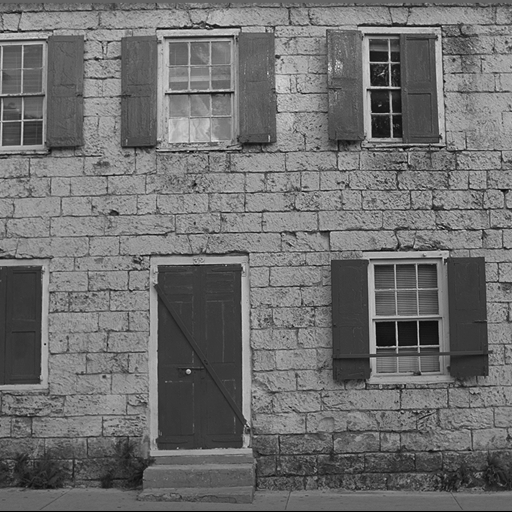
\includegraphics[width=0.20\textwidth]{kodak001.png}&\hspace{+12pt}
		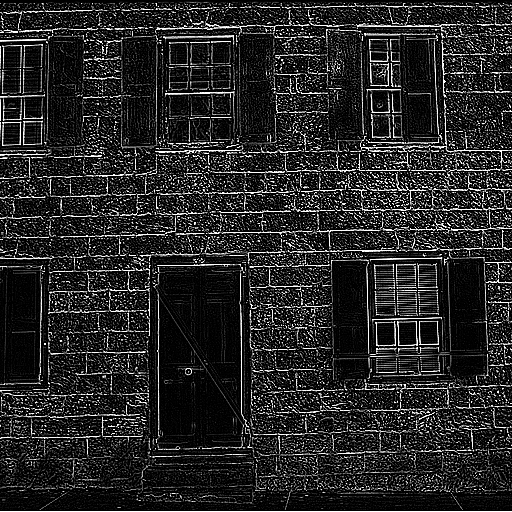
\includegraphics[width=0.20\textwidth]{kodak001_laplacian.png}&\hspace{+12pt}
		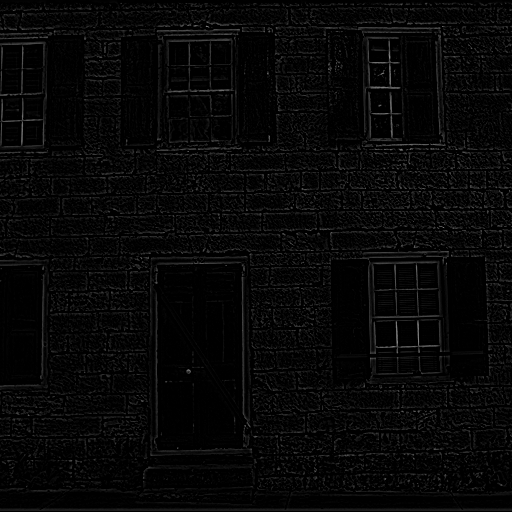
\includegraphics[width=0.20\textwidth]{kodak001_highpass.png}
		\vspace{-2pt}\\
		%%%%%%%%%
		(a) $\mathbf{X}$&\hspace{+12pt}
		(b) $\mathbf{Y}$&\hspace{+12pt}
		(c) $\mathbf{Z}$\\
		%%%%%%%%%
	\end{tabular}
	\caption{入力画像とラプラシアンフィルタリング後の出力画像、ガウシアンフィルタリングによる近似処理後の出力画像}
	\label{fig:2-4-1}
\end{figure}
%%%%%%%%%%%%%%%%%%

%%%%%%%%%%%%%%%%%%

%%%%%%%%%%%%%%%%%%
\begin{figure}[H]
	\centering
	\begin{tabular}{ccc}
		%%%%%%%%%
		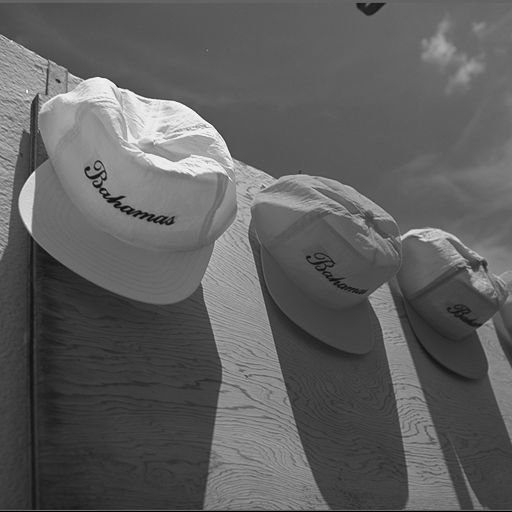
\includegraphics[width=0.20\textwidth]{kodak002.png}&\hspace{+12pt}
		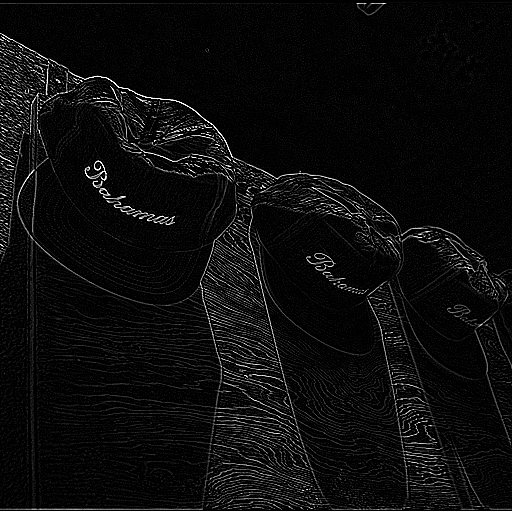
\includegraphics[width=0.20\textwidth]{kodak002_laplacian.png}&\hspace{+12pt}
		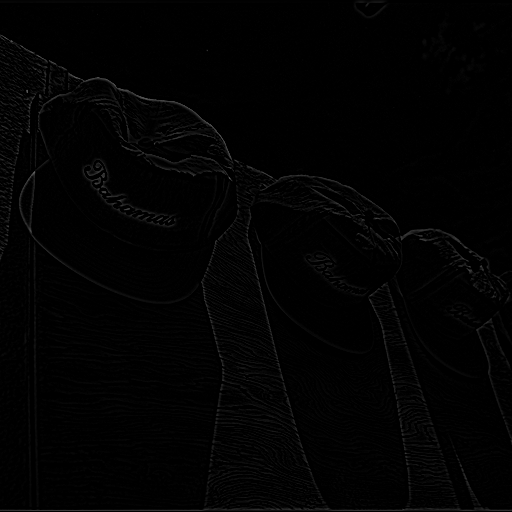
\includegraphics[width=0.20\textwidth]{kodak002_highpass.png}
		\vspace{-2pt}\\
		%%%%%%%%%
		(a) $\mathbf{X}$&\hspace{+12pt}
		(b) $\mathbf{Y}$&\hspace{+12pt}
		(c) $\mathbf{Z}$\\
		%%%%%%%%%
	\end{tabular}
	\caption{入力画像とラプラシアンフィルタリング後の出力画像、ガウシアンフィルタリングによる近似処理後の出力画像}
	\label{fig:2-4-1}
\end{figure}
%%%%%%%%%%%%%%%%%%

%%%%%%%%%%%%%%%%%%

%%%%%%%%%%%%%%%%%%
\begin{figure}[H]
	\centering
	\begin{tabular}{ccc}
		%%%%%%%%%
		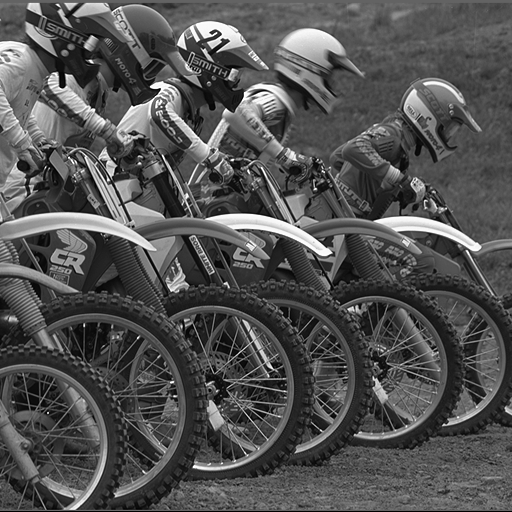
\includegraphics[width=0.20\textwidth]{kodak003.png}&\hspace{+12pt}
		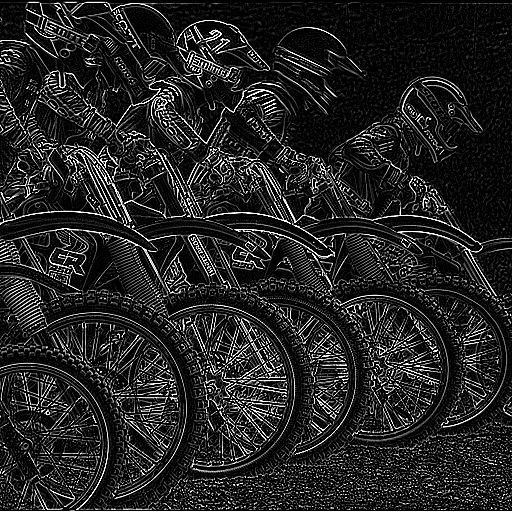
\includegraphics[width=0.20\textwidth]{kodak003_laplacian.png}&\hspace{+12pt}
		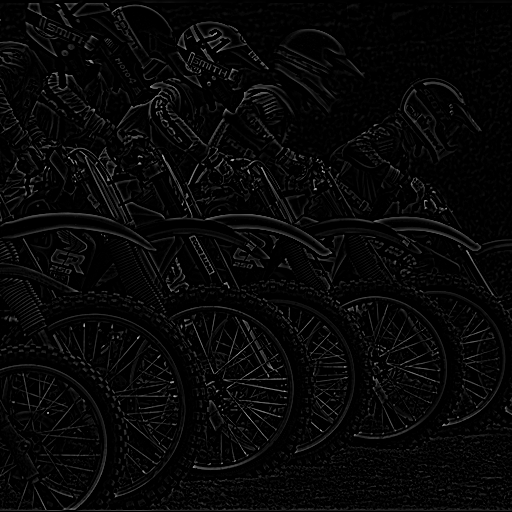
\includegraphics[width=0.20\textwidth]{kodak003_highpass.png}
		\vspace{-2pt}\\
		%%%%%%%%%
		(a) $\mathbf{X}$&\hspace{+12pt}
		(b) $\mathbf{Y}$&\hspace{+12pt}
		(c) $\mathbf{Z}$\\
		%%%%%%%%%
	\end{tabular}
	\caption{入力画像とラプラシアンフィルタリング後の出力画像、ガウシアンフィルタリングによる近似処理後の出力画像}
	\label{fig:2-4-1}
\end{figure}
%%%%%%%%%%%%%%%%%%

%%%%%%%%%%%%%%%%%%
\subsection{アンシャープマスキングによる画像のエッジ強調}
\noindent
\sizi{この節は\ref{sec:2-5}節を記述した者は必須。}

ここに、\ref{sec:2-5}節の結果と考察を示す。
図に、入力画像$\mathbf{X}$とそのエッジ成分画像$\mathbf{Y}$、アンシャープマスキングによる強調後の出力画像$\mathbf{Z}$をそれぞれ示す。ここで、ガウシアンフィルタは$k=$\rainn{}と$\sigma=$\rainn{}で設計し、アンシャープマスキングの増幅率は$p=$\rainn{}とした。
\sizi{これらの図に対する考察を述べる。}

\noindent
\sizi{同様に、他の設定における結果の表示とそれに対する考察を述べる。}

%%%%%%%%%%%%%%%%%%
% \begin{figure}[t]
% 	\centering
% 	\begin{tabular}{ccc}
% 		%%%%%%%%%
% 		\includegraphics[width=0.20\textwidth]{./figure/aa_jFigure.pdf}&\hspace{+12pt}
% 		\includegraphics[width=0.20\textwidth]{./figure/aa_jFigure.pdf}&\hspace{+12pt}
% 		\includegraphics[width=0.20\textwidth]{./figure/aa_jFigure.pdf}
% 		\vspace{-2pt}\\
% 		%%%%%%%%%
% 		(a) $\mathbf{X}$&\hspace{+12pt}
% 		(b) $\mathbf{Y}$&\hspace{+12pt}
% 		(c) $\mathbf{Z}$\\
% 		%%%%%%%%%
% 	\end{tabular}
% 	\caption{入力画像とそのエッジ成分画像、強調後の出力画像}
% 	\label{fig:2-5-1}
% \end{figure}
%%%%%%%%%%%%%%%%%%

\section{課題}
\subsection{課題1}
\noindent
\sizi{ここに調べた結果を整理して記述する。}

\subsection{課題2}
\noindent
\sizi{ここに調べた結果を整理して記述する。}

\subsection{課題3}
\noindent
\sizi{ここに調べた結果を整理して記述する。}

	
	\section{参考文献}
	\begin{enumerate}
		\renewcommand{\labelenumi}{\lbrack \arabic{enumi}\rbrack}
		\item \sizi{ここに参考文献を載せる}
		\item \sizi{ここに参考文献を載せる}
		\item \sizi{ここに参考文献を載せる}
	\end{enumerate}
	
\end{document}